\lecture{Introdução - Variáveis aleatórias}{lec_intro}

\begin{frame}
	\begin{block}{\centering\large\bfseries Parte 1}
		\centering\large\insertpart
	\end{block}
\end{frame}

\section{Introdução às comunicações digitais}

\begin{frame}
	\frametitle{Modulações analógicas e digitais}

	\begin{figure}[t]
	  \begin{center}
	    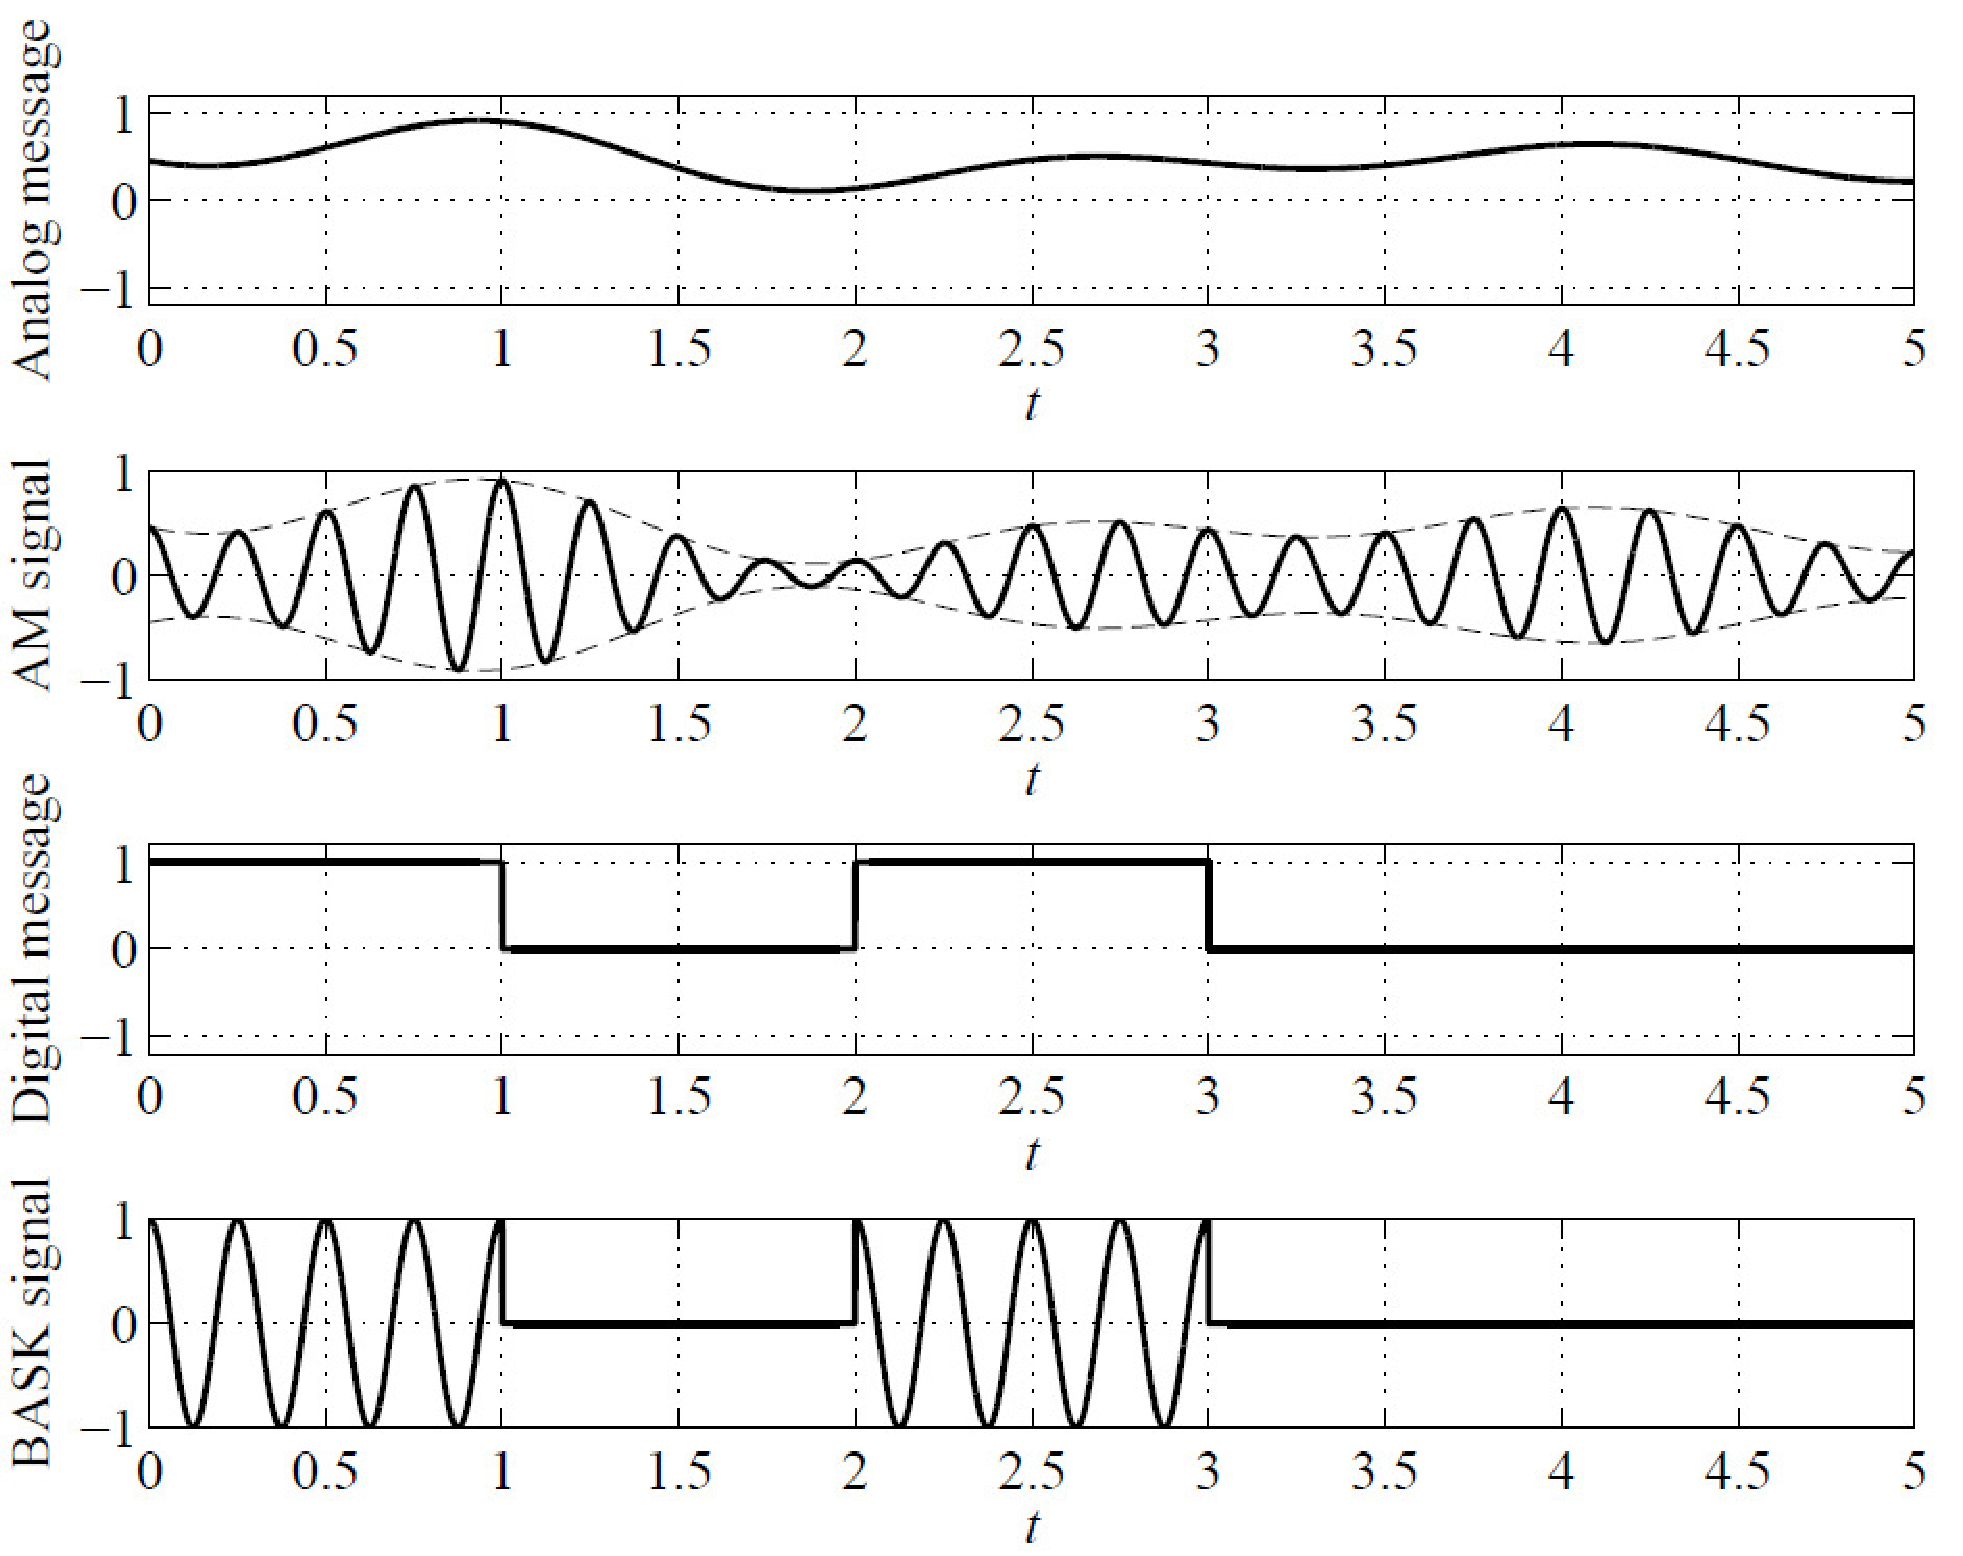
\includegraphics[width=0.77\columnwidth]{figs/fig01}
	  \end{center}
	\end{figure}

\end{frame}

\begin{frame}
    \frametitle{O que é comunicação digital?}
    
    \begin{figure}[t]
	  \begin{center}
	    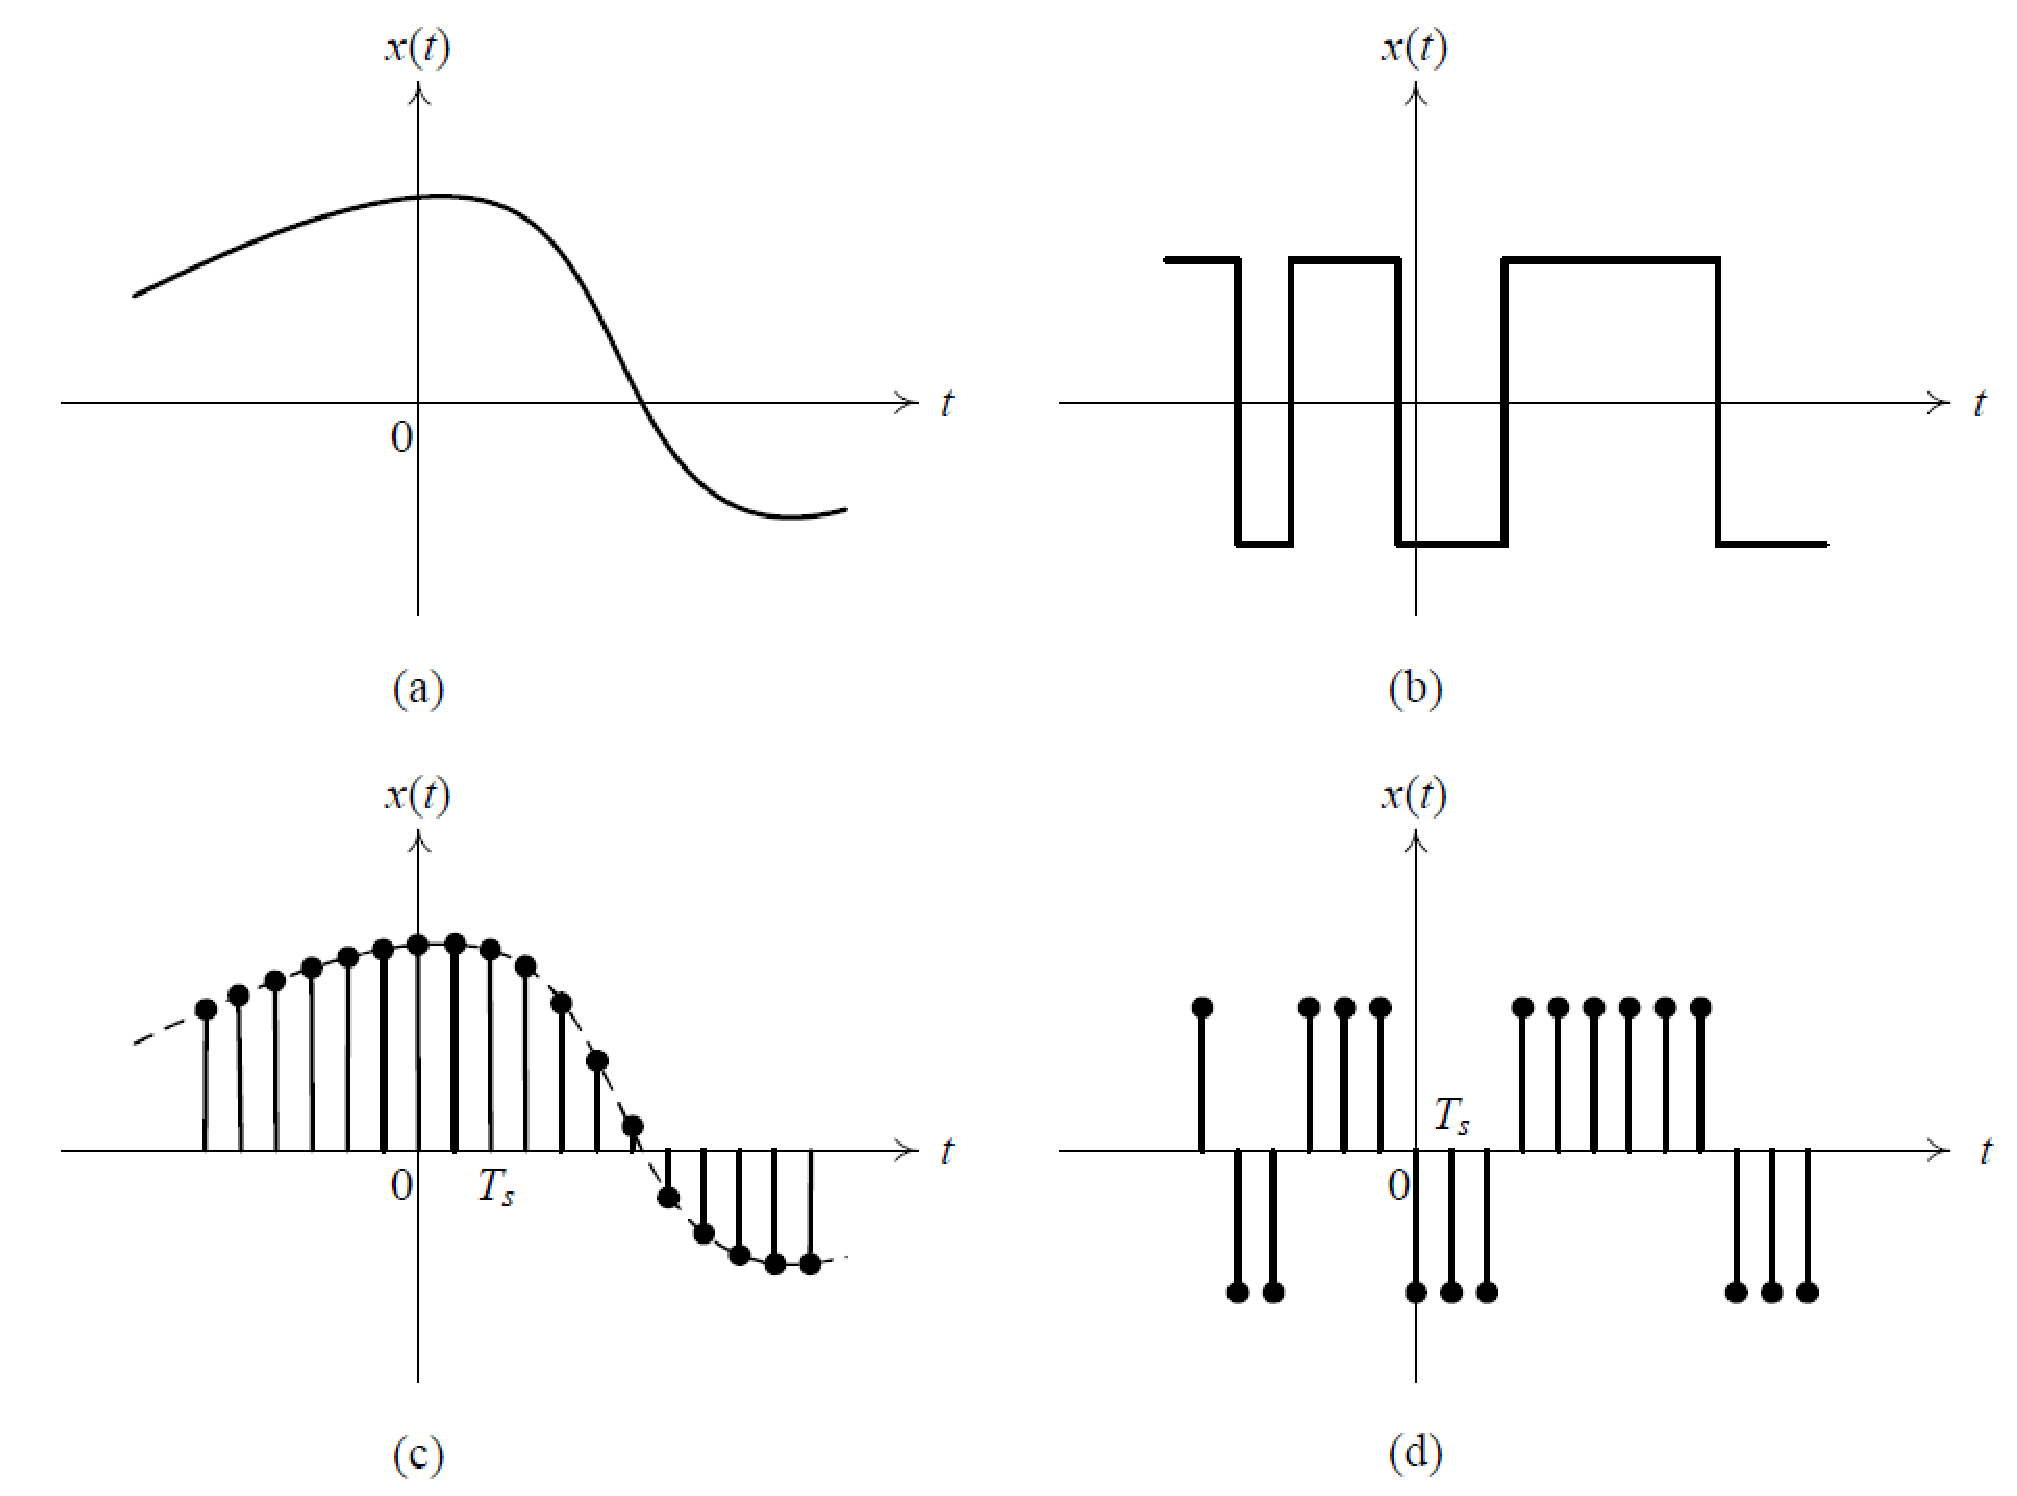
\includegraphics[width=0.77\columnwidth]{figs/fig02}
	  \end{center}
	\end{figure}
\end{frame}

\begin{frame}
    \frametitle{Por quê comunicação digital?}
    
    \begin{figure}[t]
	  \begin{center}
	    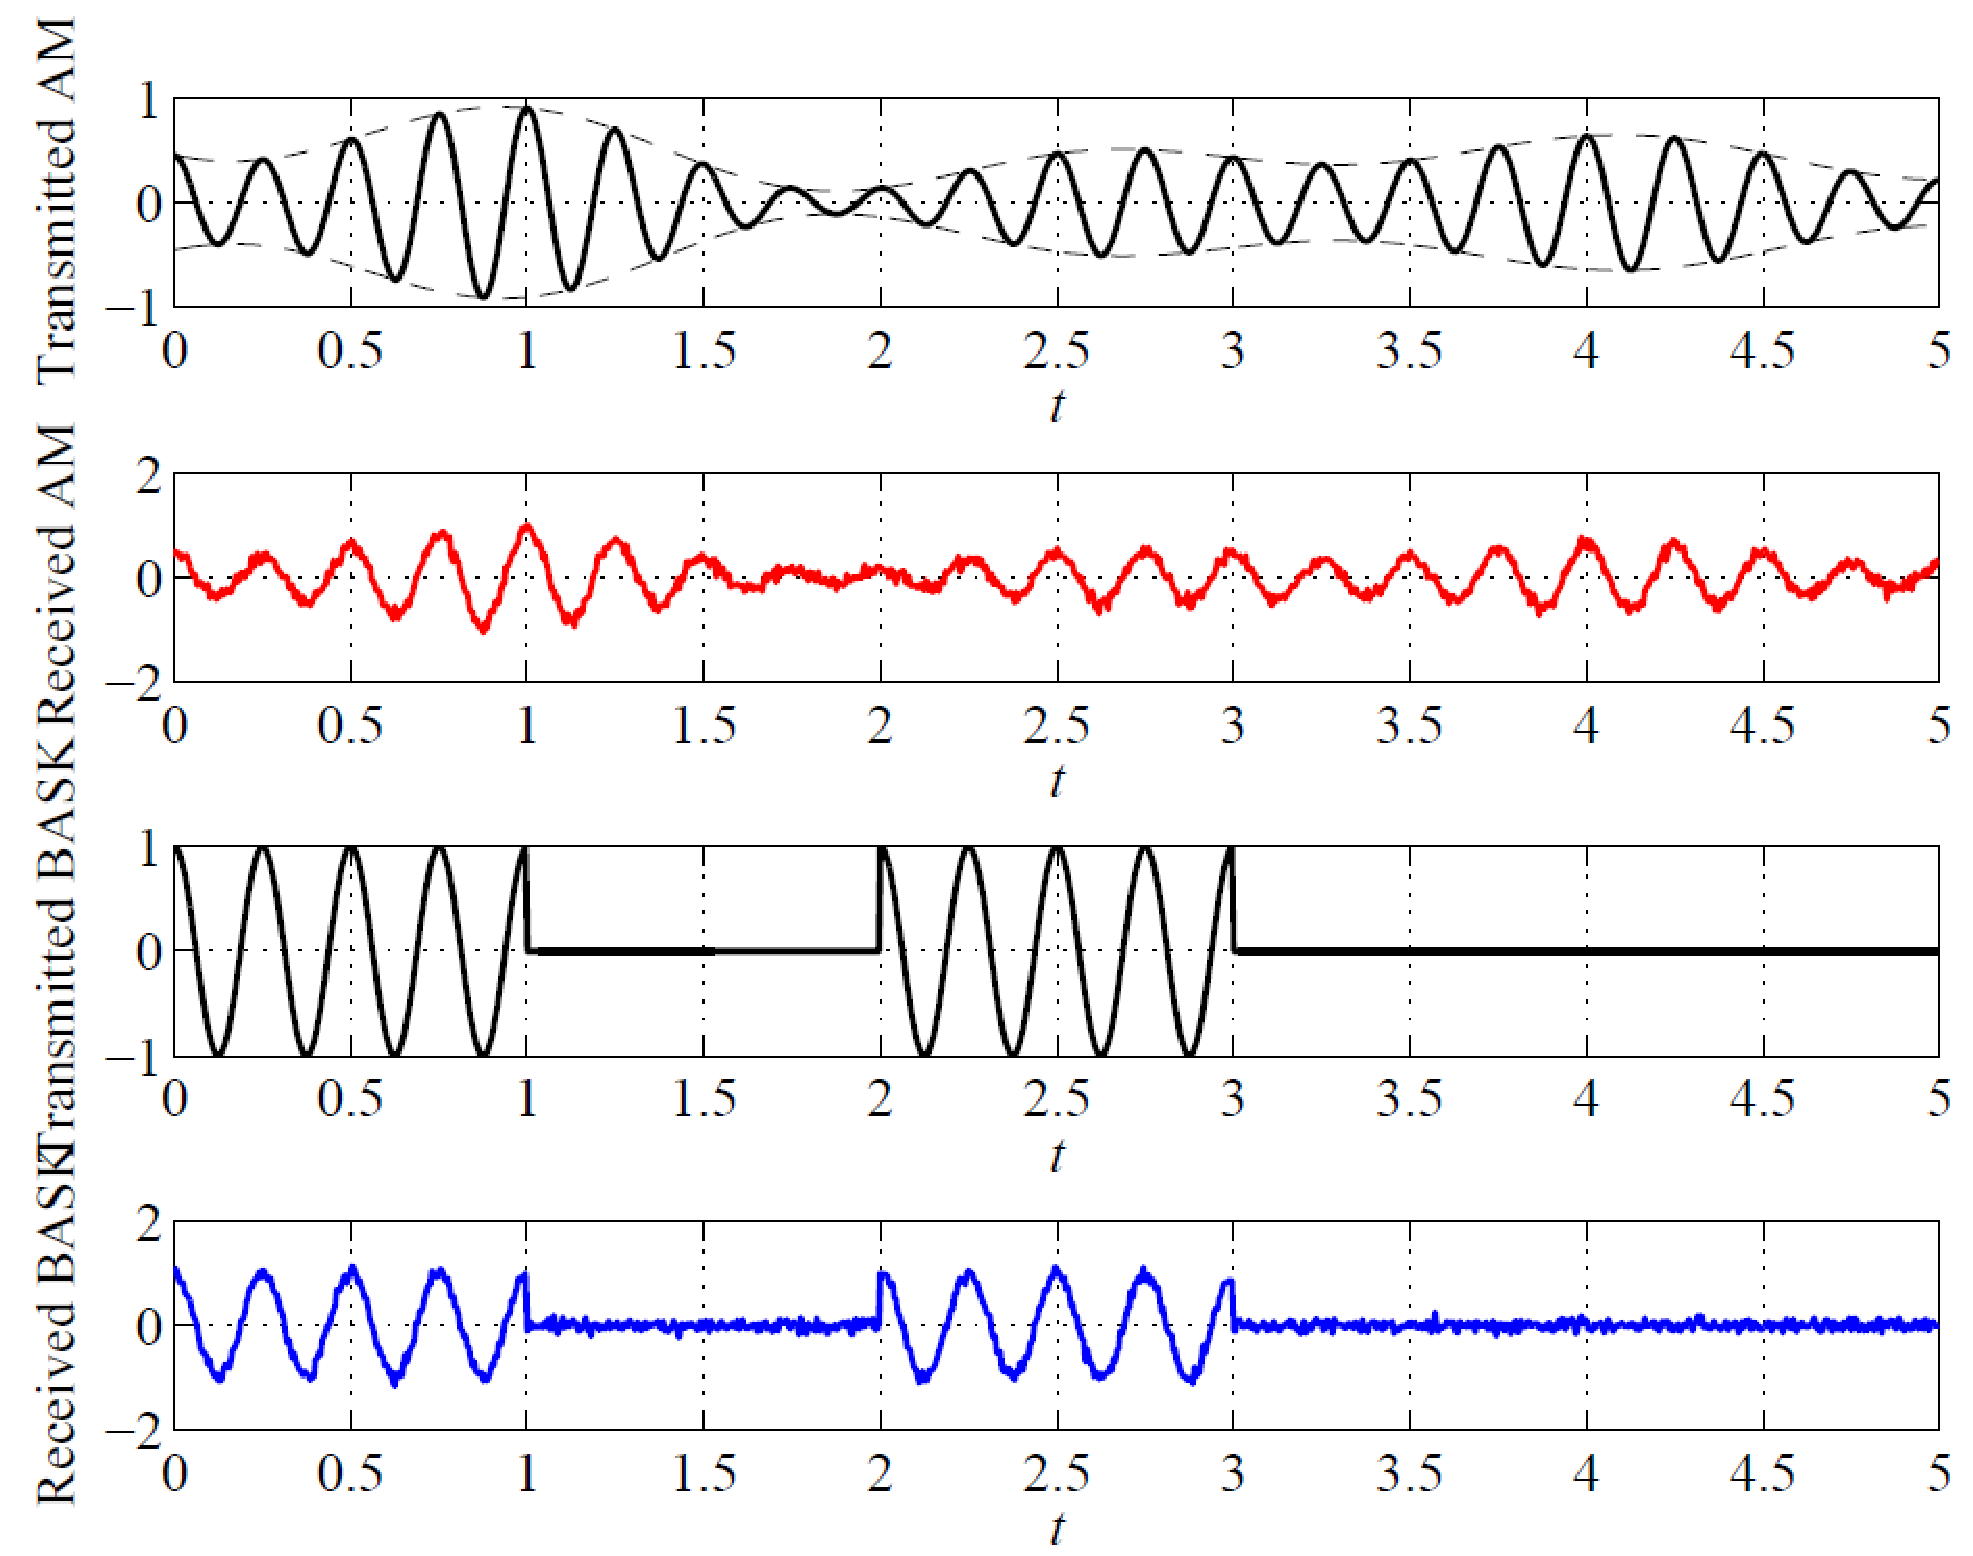
\includegraphics[width=0.77\columnwidth]{figs/fig03}
	  \end{center}
	\end{figure}
\end{frame}

\begin{frame}
    \frametitle{Por quê comunicação digital?}
    
    \begin{figure}[t]
	  \begin{center}
	    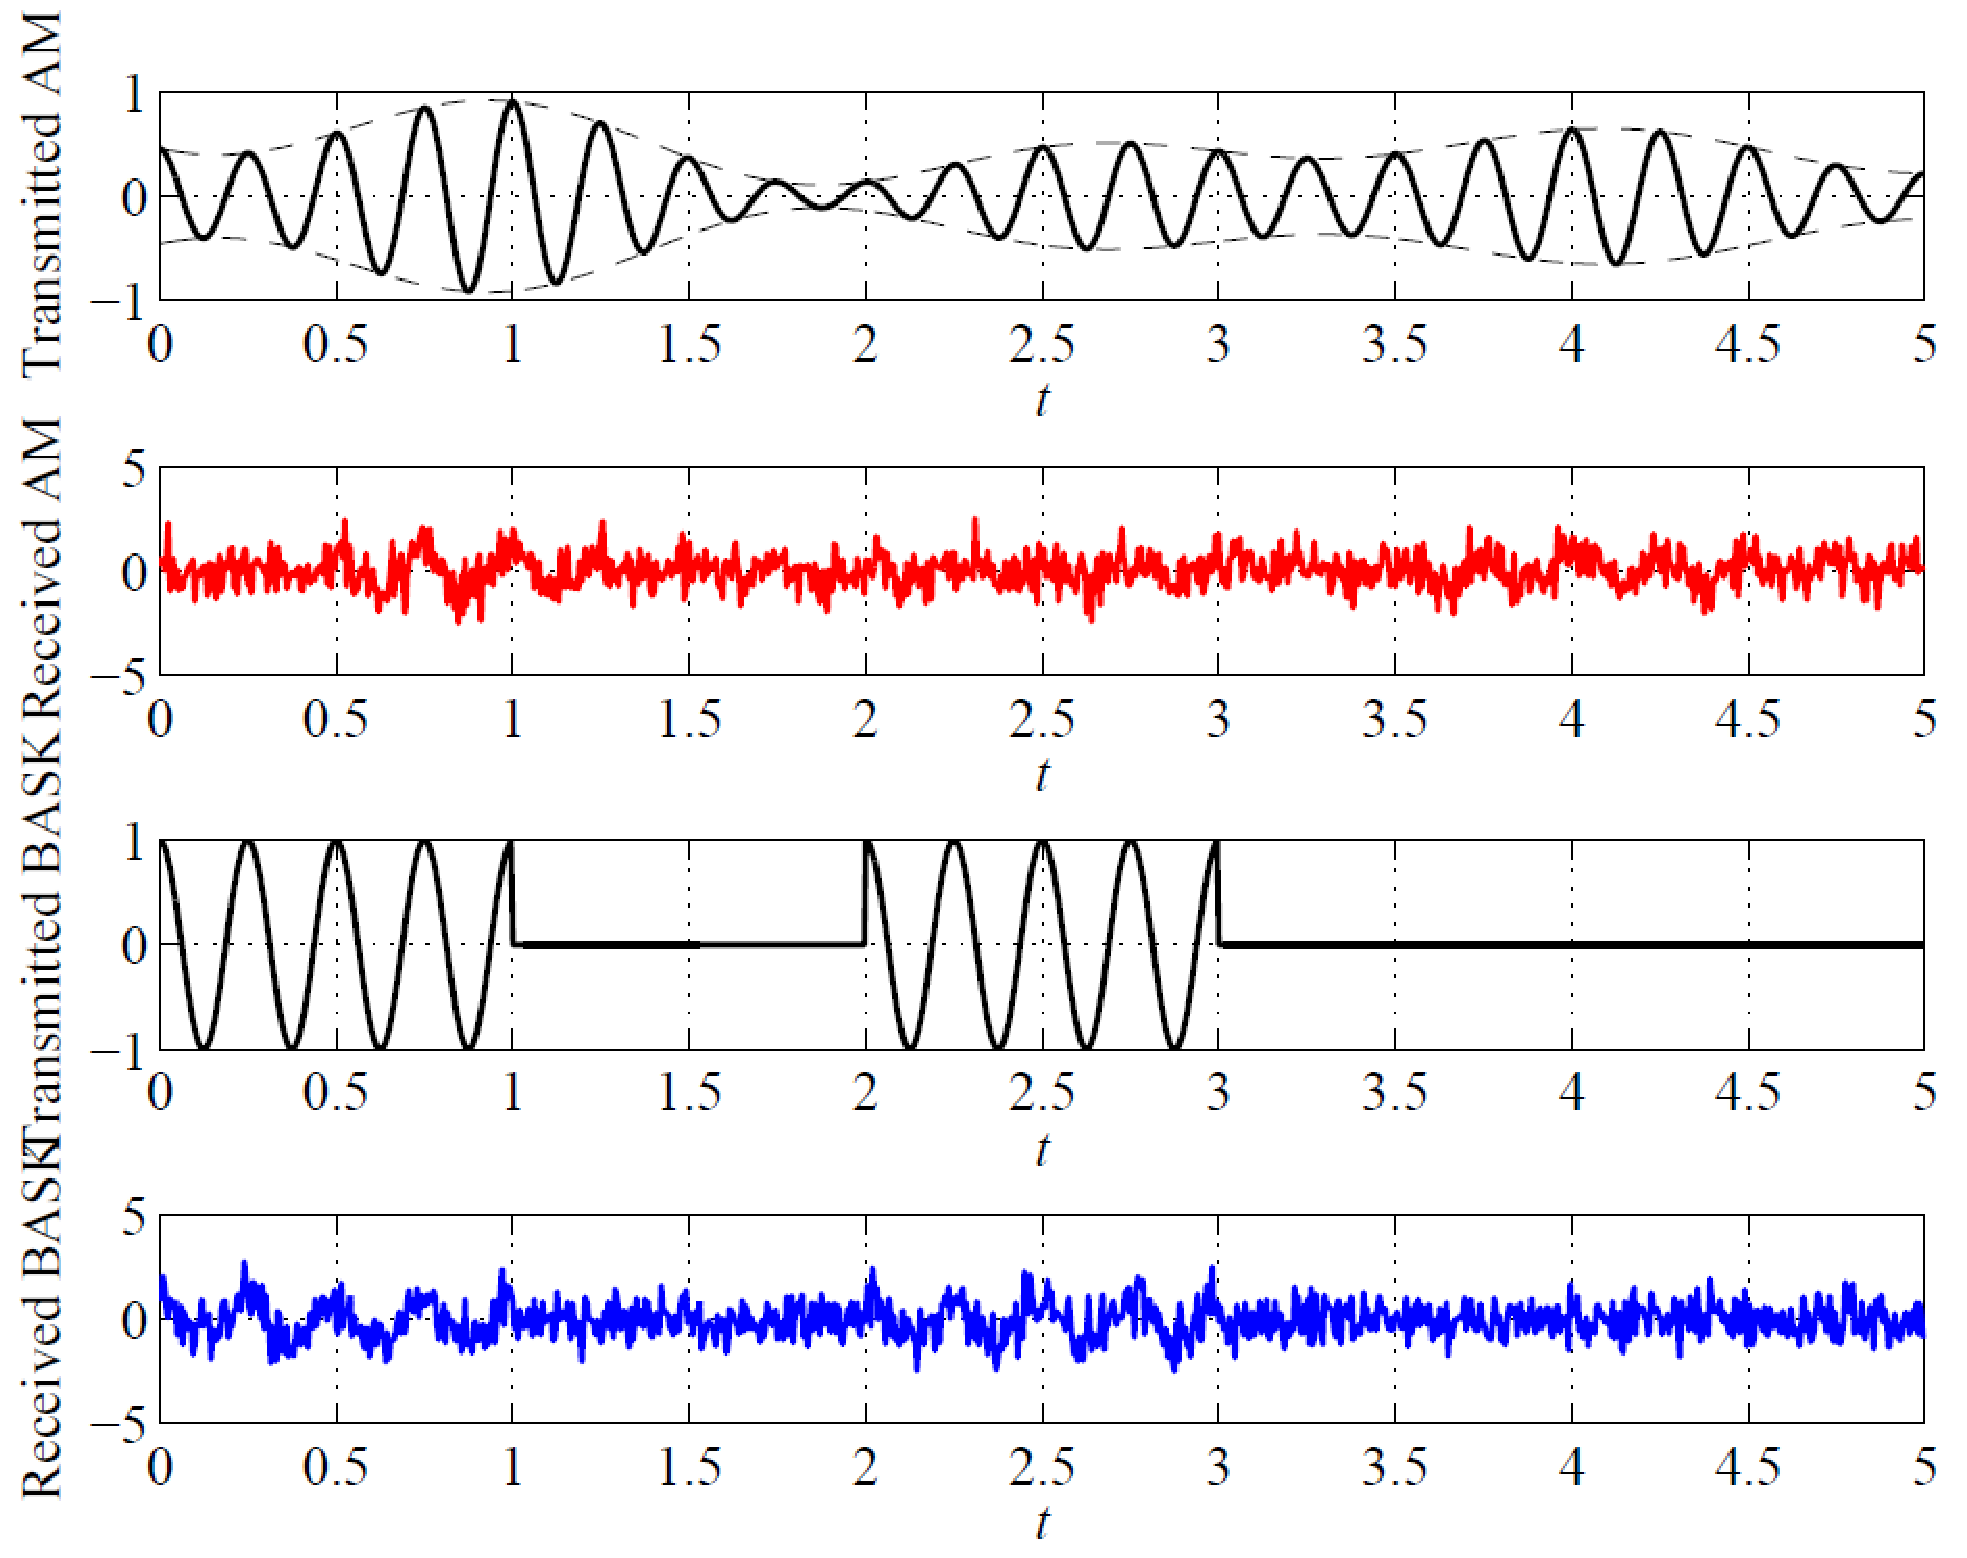
\includegraphics[width=0.77\columnwidth]{figs/fig04}
	  \end{center}
	\end{figure}
\end{frame}

\begin{frame}
    \frametitle{Repetidor regenerativo}
    
    \begin{figure}[t]
	  \begin{center}
	    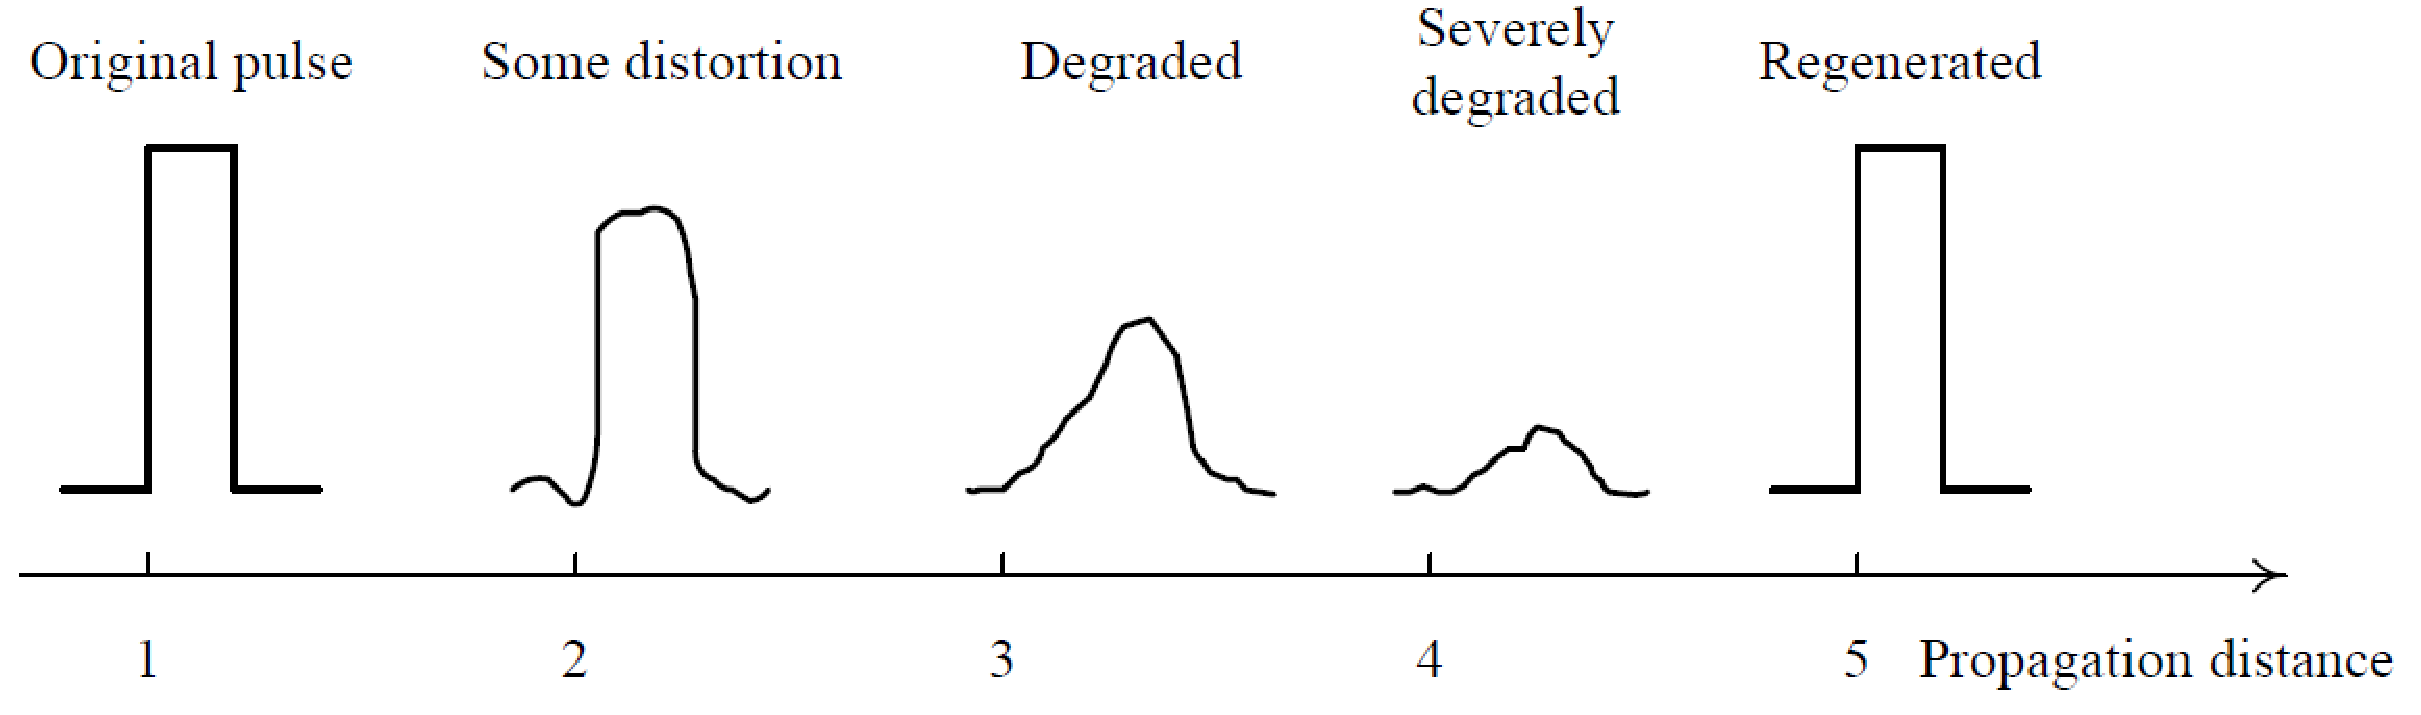
\includegraphics[width=0.77\columnwidth]{figs/fig05}
	  \end{center}
	\end{figure}
    \begin{itemize}
     \item Comunicações digitais: os sinais transmitidos pertencem a um conjunto finito de formas de onda $\Rightarrow$ O sinal distorcido pode ser recuperado para a sua forma ideal, portanto removendo totalmente o ruído.
      \item Comunicações analógicas: os sinais transmitidos são formas de onda analógicas, as quais podem assumir uma variedade infinita de formas $\Rightarrow$ Uma vez distorcido o sinal, a distorção dificilmente pode ser removida.
    \end{itemize}
\end{frame}

\begin{frame}
    \frametitle{Diagrama de blocos de um sistema de comunicação}
    
    \begin{figure}[t]
	  \begin{center}
	    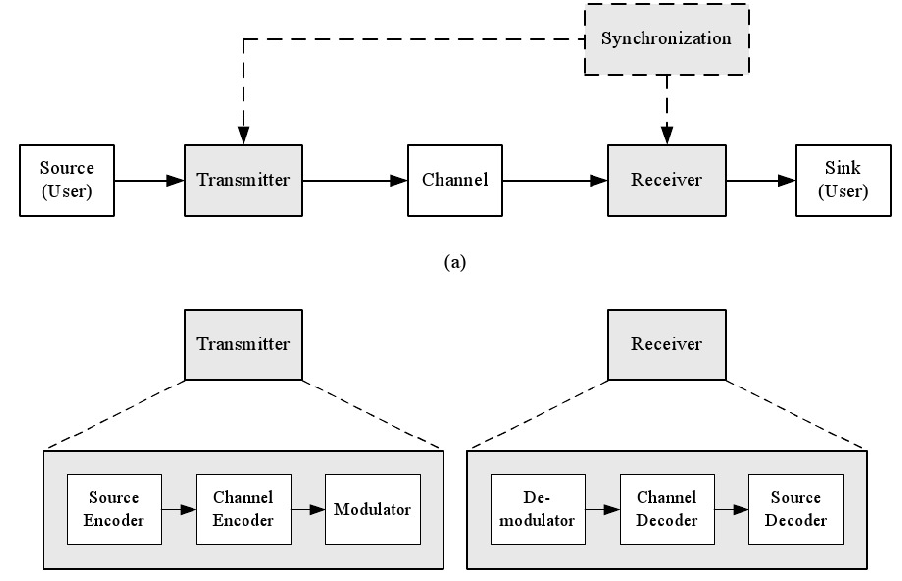
\includegraphics[width=0.77\columnwidth]{figs/fig06}
	  \end{center}
	\end{figure}
\end{frame}

\begin{frame}
    \frametitle{Digital vs. Analógico}
    
    \begin{itemize}
     \item Vantagens:
	\begin{itemize}
	 \item Sinais digitais são mais fáceis de serem regenerados.
	  \item Circuitos digitais estão menos sujeitos a distorção e interferência.
	  \item Circuitos digitais são mais confiáveis e podem ser produzidos a um custo menor do que circuitos analógicos.
	  \item A implementação de hardware digital é mais flexível que a de hardware analógico.
	  \item Sinais digitais podem se beneficiar de técnicas de processamento digital de sinais.
	\end{itemize}
     \item Desvantagens:
	\begin{itemize}
	 \item Processamento de sinais mais intenso. 
	  \item A sincronização é uma questão crucial.
	  \item Requer maior banda de transmissão.
	  \item Degradação não-suave.
	\end{itemize}
    \end{itemize}
\end{frame}

\section{Probabilidade e variáveis aleatórias}

\begin{frame}
    \frametitle{Espaço amostral e probabilidade}
    
    \begin{itemize}
     \item \textit{Experimento aleatório}: seu resultado, por algum motivo, não pode ser previsto com absoluta certeza.
      \item Exemplos: arremesso de um dado ou moeda, ou retirada de uma carta de uma pilha.
      \item \textit{Espaço amostral}: o conjunto de todos os possíveis resultados, denotado por $\Omega$. Os resultados individuais são denotados por $\omega$, onde $\omega \in \Omega$.
      \item Um espaço amostral pode ser \textit{discreto} ou \textit{contínuo}.
      \item \textit{Eventos} são subconjuntos do espaço amostral para os quais medidas de suas ocorrências, chamadas de probabilidades, podem ser definidas ou determinadas.
    \end{itemize}
\end{frame}

\begin{frame}
    \frametitle{Os três axiomas da probabilidade}
    
    \begin{itemize}
     \item Para um espaço amostral discreto $\Omega$, define-se a medida de probabilidade $P$ em $\Omega$ como uma função que assinala valores não-negativos a todos os eventos, denotados por $E$, em $\Omega$, tal que as seguintes condições são satisfeitas:
    \begin{itemize}
     \item Axioma 1: $0 \leq P(E) \leq 1$ para todo $E \in \Omega$.
     \item Axioma 2: $P(\Omega) = 1$
     \item Axioma 3: Para eventos mutuamente exclusivos, i.e., $E_i \cap E_j = \oslash \; \forall i \neq j$, tem-se que $P(\bigcup\limits_{i=1}^{\infty} E_i) = \sum\limits_{i=1}^{\infty} P(E_i)$
    \end{itemize}

    \end{itemize}
\end{frame}

\begin{frame}
    \frametitle{Propriedades importantes}
    
    \begin{enumerate}
      \item $P(E^C) = 1 - P(E)$, onde $E^C$ denota o complemento de $E$. Esta propriedade implica que $P(E^C) + P(E) = 1$, ou seja, algo tem que ocorrer.
      \item $P(\oslash) = 0$, novamente, alguma coisa tem que ocorrer.
      \item $P(E_1 \cup E_2) = P(E_1) + P(E_2) - P(E_1 \cap E_2)$. Note que se dois eventos $E_1$ e $E_2$ são mutuamente exclusivos então $P(E_1 \cup E_2) = P(E_1) + P(E_2)$.
      \item Se $E_1 \subseteq E_2$ então $P(E_1) \leq P(E_2)$. 
    \end{enumerate}
\end{frame}


\begin{frame}
    \frametitle{Probabilidade condicional}
    
    \begin{itemize}
      \item Observamos o evento $E_1$, mas na verdade estamos interessados no evento $E_2$: o conhecimento de que $E_1$ ocorreu altera a probabilidade de que $E_2$ ocorra.
      \item Se antes tinha-se $P(E_2)$, agora tem-se $P(E_2 | E_1)$, ou seja, a probabilidade de que $E_2$ ocorra dado que $E_1$ ocorreu.
      \item A probabilidade condicional é dada por
      \begin{equation}
	  P(E_2 | E_1) = \begin{cases}
			    \frac{P(E_2 \cap E_1)}{P(E_1)} \, , \quad \textrm{se} & P(E_1) \neq 0 \\
			     0 & c.c.
	                 \end{cases}
      \end{equation}

      \item Se $P(E_2| E_1) = P(E_2)$, ou $P(E_2 \cap E_1) = P(E_1) P(E_2)$, então $E_1$ e $E_2$ são ditos \textit{estatísticamente independentes}. 
      \item Regra de Bayes:
	\begin{equation}
	    P(E_2 | E_1) = \frac{P(E_1 | E_2) P(E_2)}{P(E_1)}
	\end{equation}
    \end{itemize}
\end{frame}


\begin{frame}
    \frametitle{Teorema da probabilidade total}
    
    \begin{itemize}
      \item Os eventos $\{E\}_{i=1}^n$ particionam o espaço amostral $\Omega$ se:
      \begin{itemize}
       \item $\bigcup\limits_{i=1}^n E_i = \Omega$
	\item $E_i \cap E_j = \oslash$ para todo $1 \leq i, \; j \leq n$ e $i \neq j$
      \end{itemize}
      \item Se um evento $A$ tem probabilidades condicionais $\{P(A|E_i)\}_{i=1}^n$, $P(A)$ pode ser obtido por
      \begin{equation}
	  P(A) = \sum\limits_{i=1}^n P(E_i) P(A | E_i)
      \end{equation}
      \item Regra de Bayes
      \begin{equation}
	  P(E_i | A) = \frac{P(A | E_i) P(E_i)}{P(A)} = \frac{P(A | E_i) P(E_i)}{\sum\limits_{j=1}^n P(A | E_j) P(E_j)}
      \end{equation}

    \end{itemize}
\end{frame}

\begin{frame}
    \frametitle{Variáveis aleatórias}
    
    \begin{figure}[t]
	  \begin{center}
	    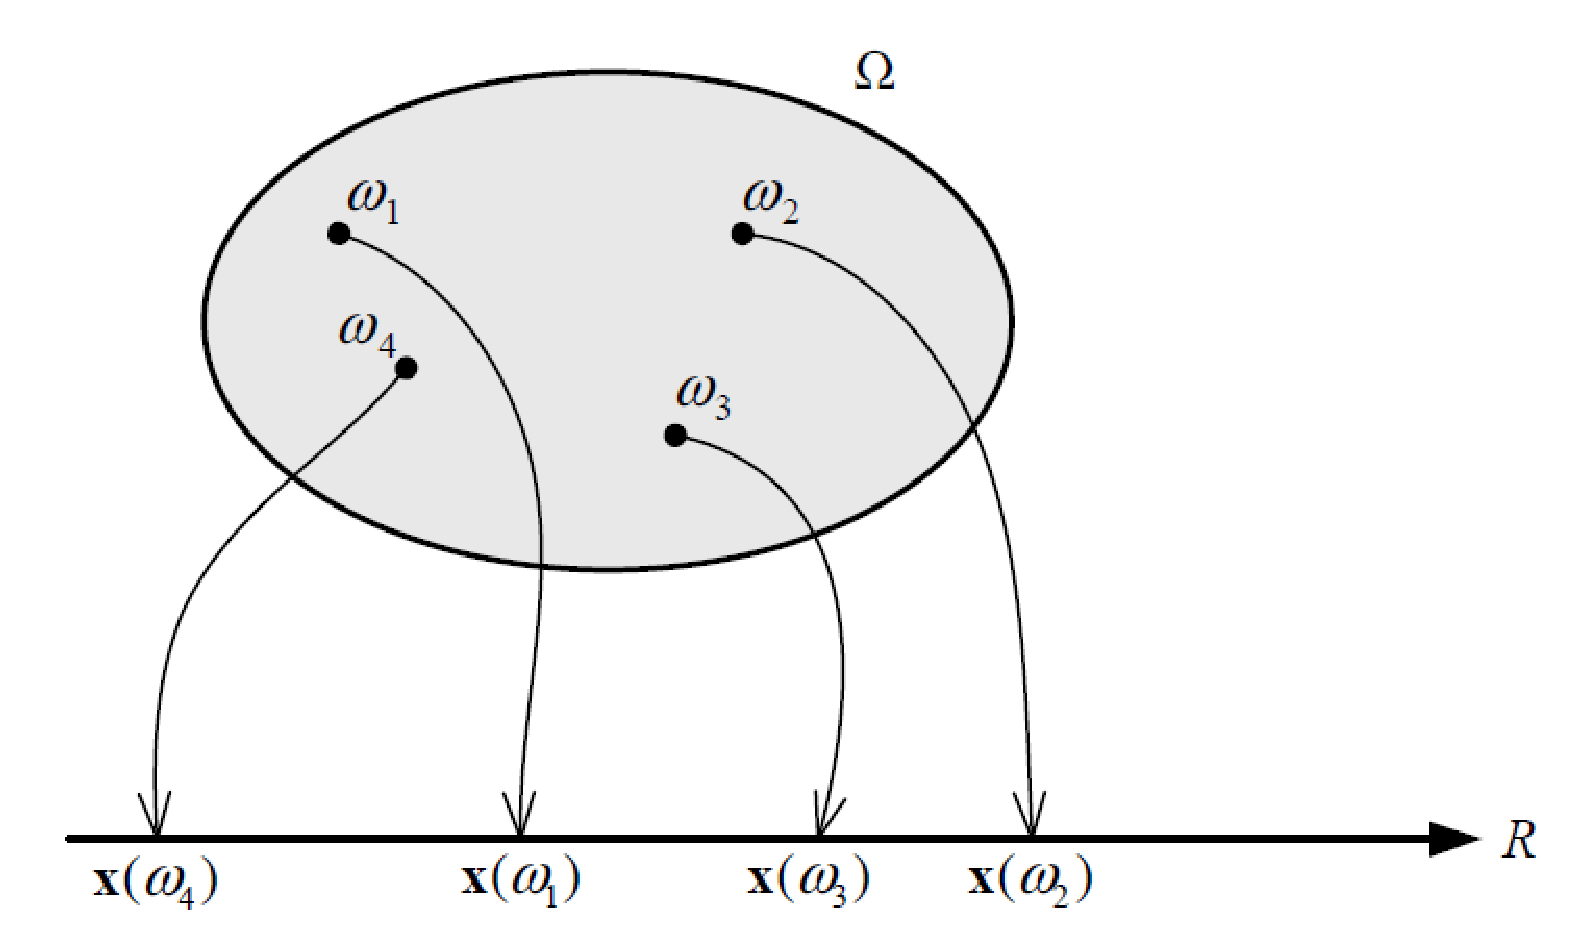
\includegraphics[width=0.6\columnwidth]{figs/fig07}
	  \end{center}
	\end{figure}

    \begin{itemize}
     \item Uma variável aleatória é um \textit{mapeamento} do espaço amostral $\Omega$ ao conjunto de números reais.
      \item Vamos expressar as variáveis aleatórias em negrito, i.e., $\mathbf{x}$, $\mathbf{y}$, etc., enquanto valores individuais ou específicos do mapeamento $\mathbf{x}$ são denotados por $\mathbf{x}(\omega)$.
    \end{itemize}

\end{frame}

\begin{frame}
    \frametitle{Função Distribuição de Probabilidade (CDF)}
    
    \begin{itemize}
      \item A CDF fornece uma descrição completa da variável aleatória. Ela é definida como:

      \begin{equation}
	  F_{\mathbf{x}}(x) = P(\omega \in \Omega \, | \, \mathbf{x}(\omega) \leq x) = P(\mathbf{x} \leq x) \, .
      \end{equation}
      
      \item A CDF possui as seguintes propriedades:
      \begin{itemize}
       \item $0 \leq F_{\mathbf{x}}(x) \leq 1$
	\item $F_{\mathbf{x}}(x)$ é não decrescente: $F_{\mathbf{x}}(x_1) \leq F_{\mathbf{x}}(x_2)$ se $x_1 \leq x_2$
	\item $F_{\mathbf{x}}(-\infty) = 0$ e $F_{\mathbf{x}}(+\infty) = 1$
	\item $P(a < \mathbf{x} \leq b) = F_{\mathbf{x}}(b) - F_{\mathbf{x}}(a)$
      \end{itemize}
    
    \end{itemize}
\end{frame}

\begin{frame}
    \frametitle{Exemplos de CDFs típicas - I}

    \begin{itemize}
     \item Uma variável aleatória pode ser \textit{discreta}, \textit{contínua} ou \textit{mista}.
    \end{itemize}

    \begin{figure}[t]
	  \begin{center}
	    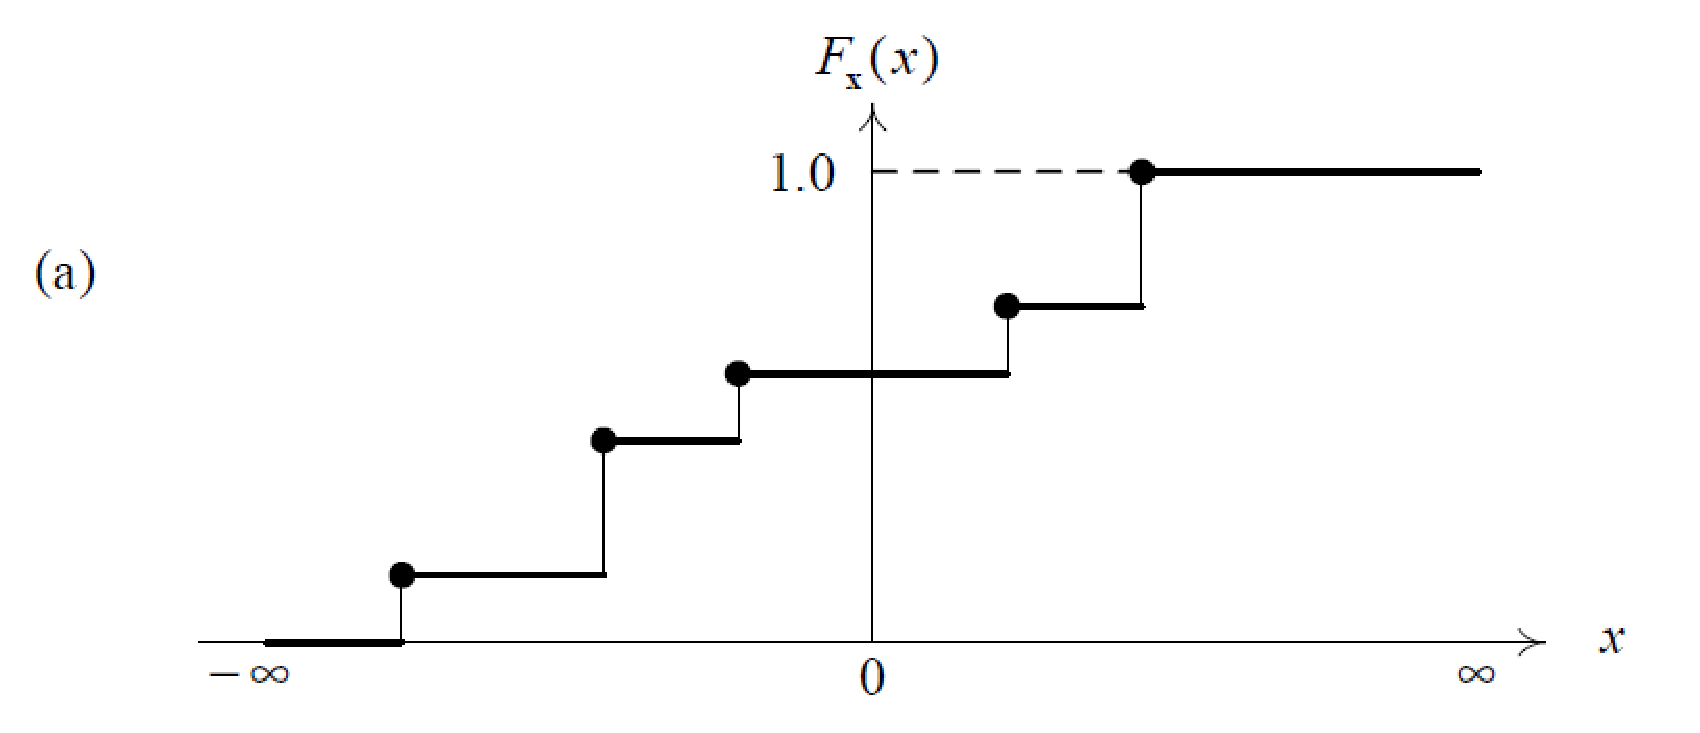
\includegraphics[width=0.77\columnwidth]{figs/fig08}
	  \end{center}
	\end{figure}
    
\end{frame}

\begin{frame}
    \frametitle{Exemplos de CDFs típicas - II}

    \begin{figure}[t]
	  \begin{center}
	    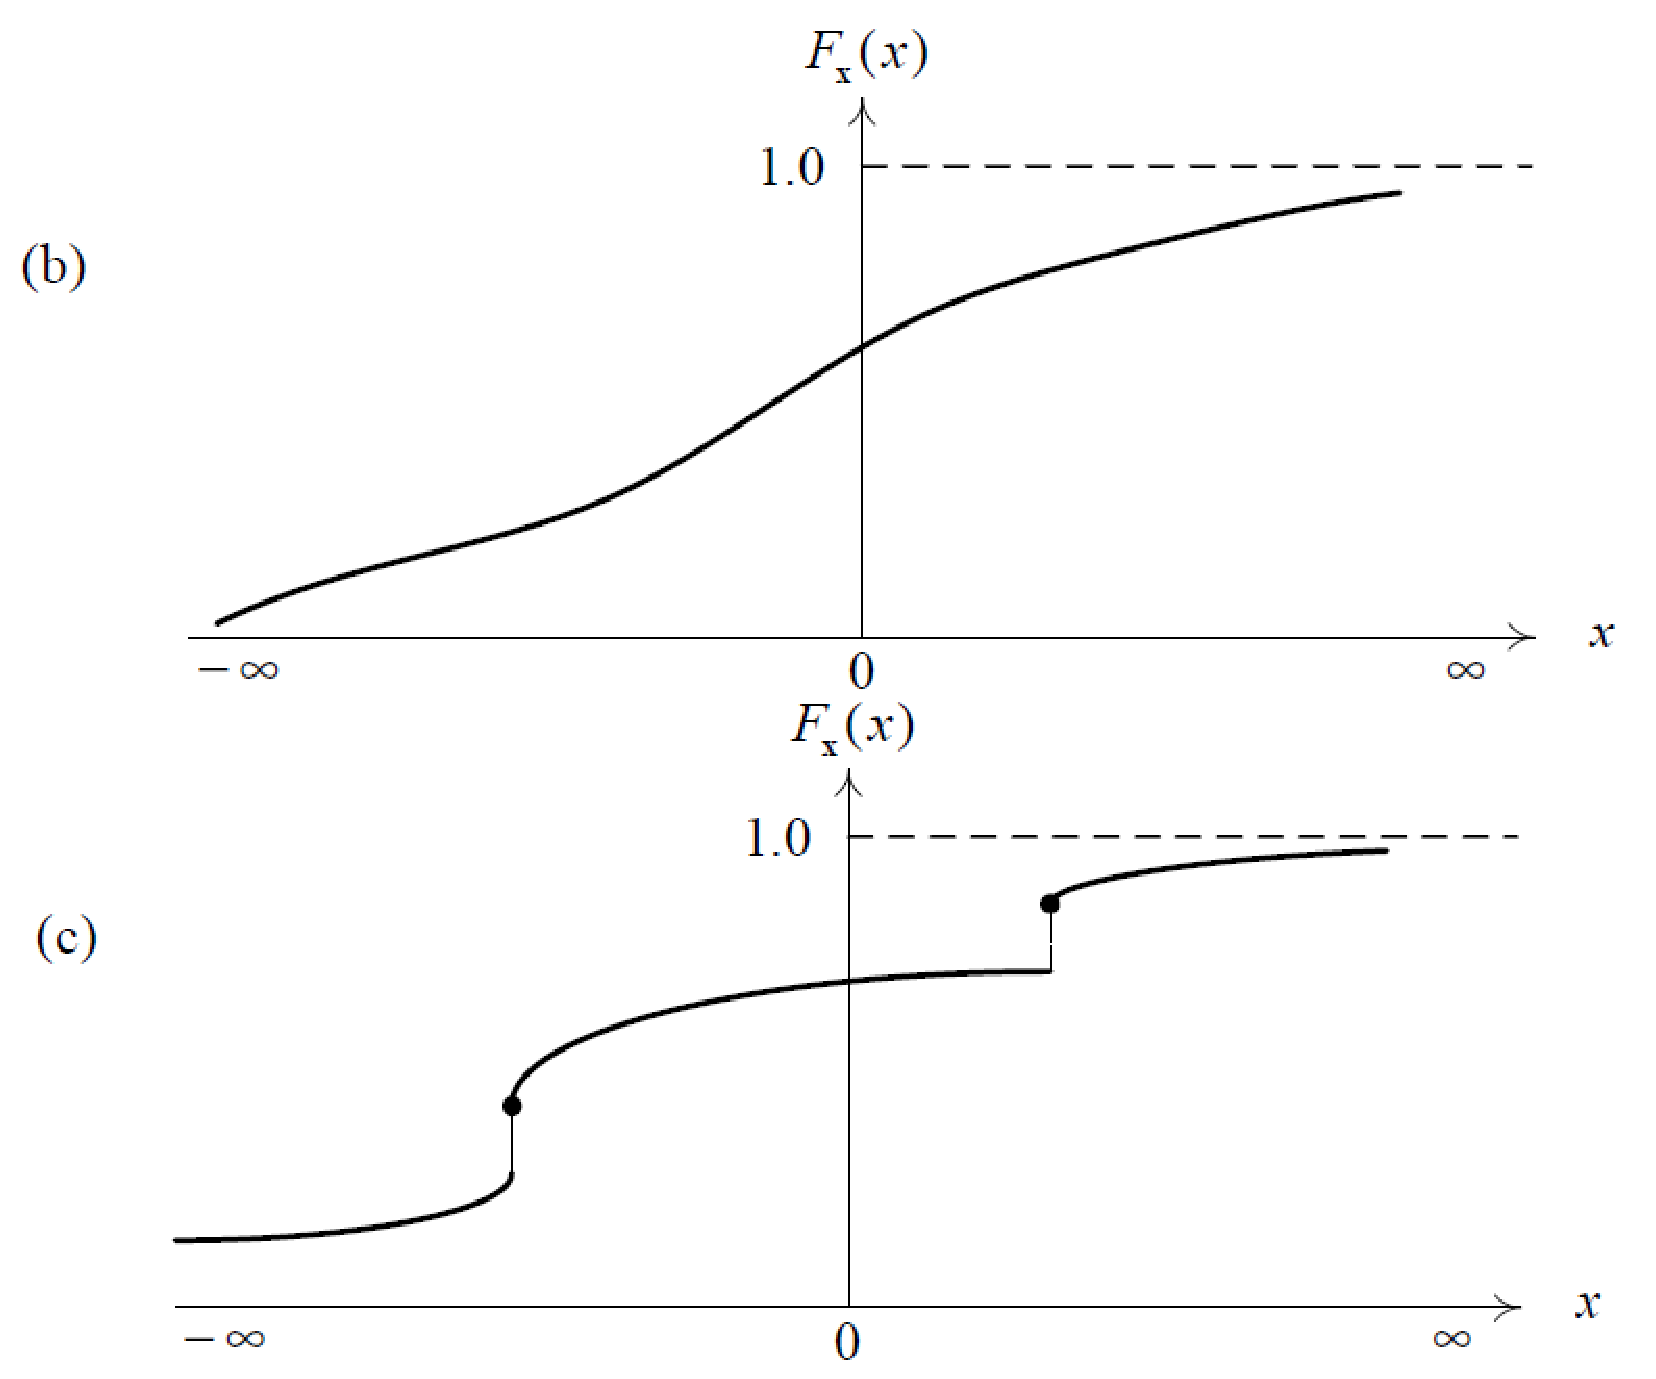
\includegraphics[width=0.7\columnwidth]{figs/fig09}
	  \end{center}
	\end{figure}
    
\end{frame}

\begin{frame}
    \frametitle{Função Densidade de Probabilidade (PDF)}
    
    \begin{itemize}
      \item A PDF é definida como a derivada da CDF:

      \begin{equation}
	  f_{\mathbf{x}}(x) = \frac{\mathrm{d} F_{\mathbf{x}}(x)}{ \mathrm{d} x} \, ; \quad F_{\vax}(x) = \int_{-\infty}^{x} f_{\vax}(u) du
      \end{equation}

      \item Segue que:
      \begin{align}
	  P(x_1 \leq \mathbf{x} \leq x_2) &= P(\mathbf{x} \leq x_2) - P(\mathbf{x} \leq x_1) \\
	  &= F_{\mathbf{x}}(x_2) - F_{\mathbf{x}}(x_1) = \int_{x_1}^{x_2}  f_{\mathbf{x}}(x)  \mathrm{d} x \, .
      \end{align}
      
      \item A PDF possui as seguintes propriedades:
      \begin{itemize}
       \item $f_{\mathbf{x}}(x) \geq 0$
	\item $\int_{-\infty}^{\infty} f_{\mathbf{x}}(x) \mathrm{d} x = 1$
	\item Em geral, $P(\mathrm{x} \in \mathcal{A}) = \int_{\mathcal{A}} f_{\mathbf{x}}(x) \mathrm{d} x$
      \end{itemize}

      \item Para variáveis aleatórias discretas é mais comum definir a função de probabilidade de massa (pmf): $p_i = P(\mathbf{x} = x_i)$.

      \item Note que, para todo $i$, temos que $p_i \geq 0$ e $\sum\limits_i p_i = 1$.
    
    \end{itemize}
\end{frame}

\begin{frame}
    \frametitle{Variável Aleatória Gaussiana}

    \begin{figure}[t]
	  \begin{center}
	    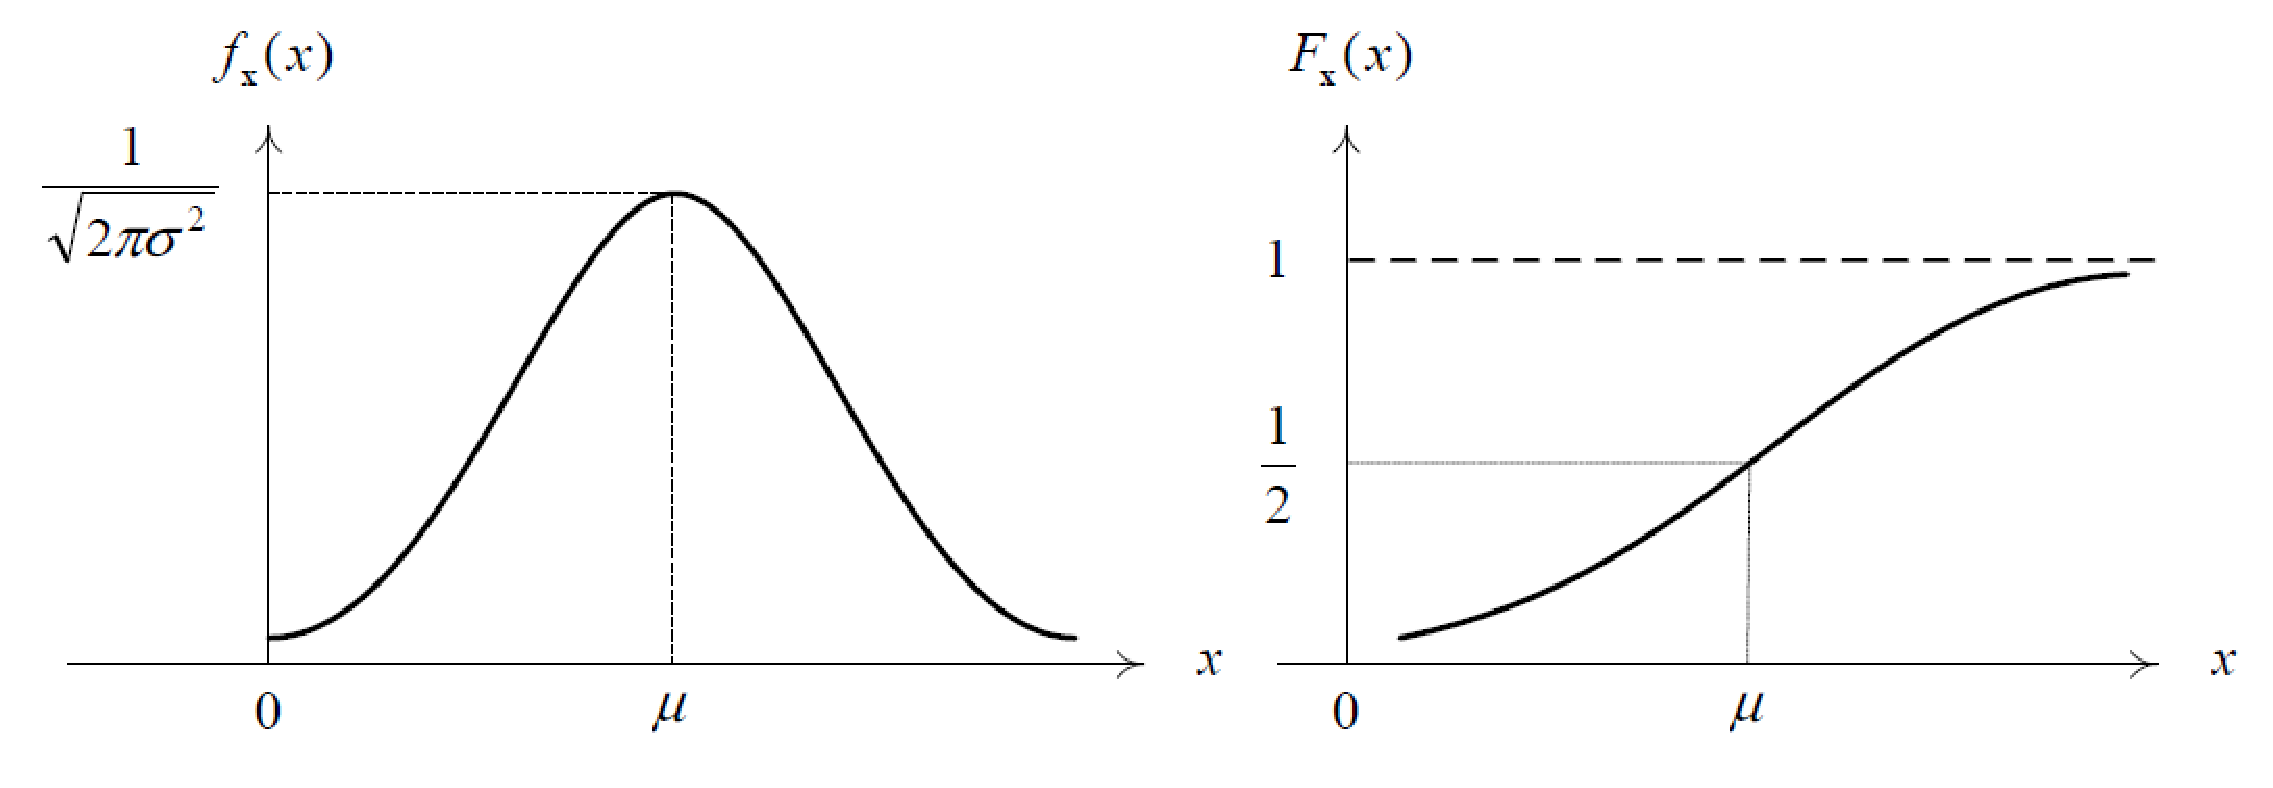
\includegraphics[width=0.77\columnwidth]{figs/fig13}
	  \end{center}
	\end{figure}

    \begin{itemize}
     \item É uma variável aleatória contínua cuja PDF é dada por:

      \begin{equation}
	  f_{\mathbf{x}}(x) = \frac{1}{\sqrt{2\pi\sigma^2}} \exp \left\{-\frac{(x-\mu)^2}{2\sigma^2}\right\} \, ,
      \end{equation}

      onde $\mu$ e $\sigma^2$ são parâmetros. É usualmente denotada por $\mathcal{N}(\mu,\sigma^2)$.
      \item É a variável aleatória mais importante e mais freqüentemente encontrada na área de comunicações.
    \end{itemize}
   
\end{frame}

\begin{frame}
    \frametitle{Variável Aleatória Gaussiana}

    \begin{itemize}
     \item Funções auxiliares:
      \begin{align}
	   \mathrm{erf}(x) &= \frac{2}{\sqrt{\pi}} \int_0^x e^{-t^2} dt \\
	   \mathrm{erfc}(x) &= \frac{2}{\sqrt{\pi}} \int_x^{\infty} e^{-t^2} dt  = 1 - \mathrm{erf}(x) \\
	   \mathrm{Q}(x) &= \frac{1}{\sqrt{2\pi}} \int_x^{\infty} e^{-t^2/2} dt  = \frac{1}{2}\mathrm{erfc}\left(\frac{x}{\sqrt{2}}\right)
      \end{align}

     \item CDF Gaussiana:

      \begin{align}
	  F_{\mathbf{x}}(x) &= \int_{-\infty}^x \frac{1}{\sqrt{2\pi\sigma^2}} \exp \left\{-\frac{(t-\mu)^2}{2\sigma^2}\right\} dt \\
	  F_{\mathbf{x}}(x) &= 1 - \frac{1}{2}\mathrm{erfc}\left( \frac{x - \mu}{\sqrt{2}\sigma} \right)
      \end{align}

    \end{itemize}

\end{frame}

\begin{frame}
    \frametitle{Variável Aleatória Gaussiana}

    \begin{figure}[t]
	  \begin{center}
	    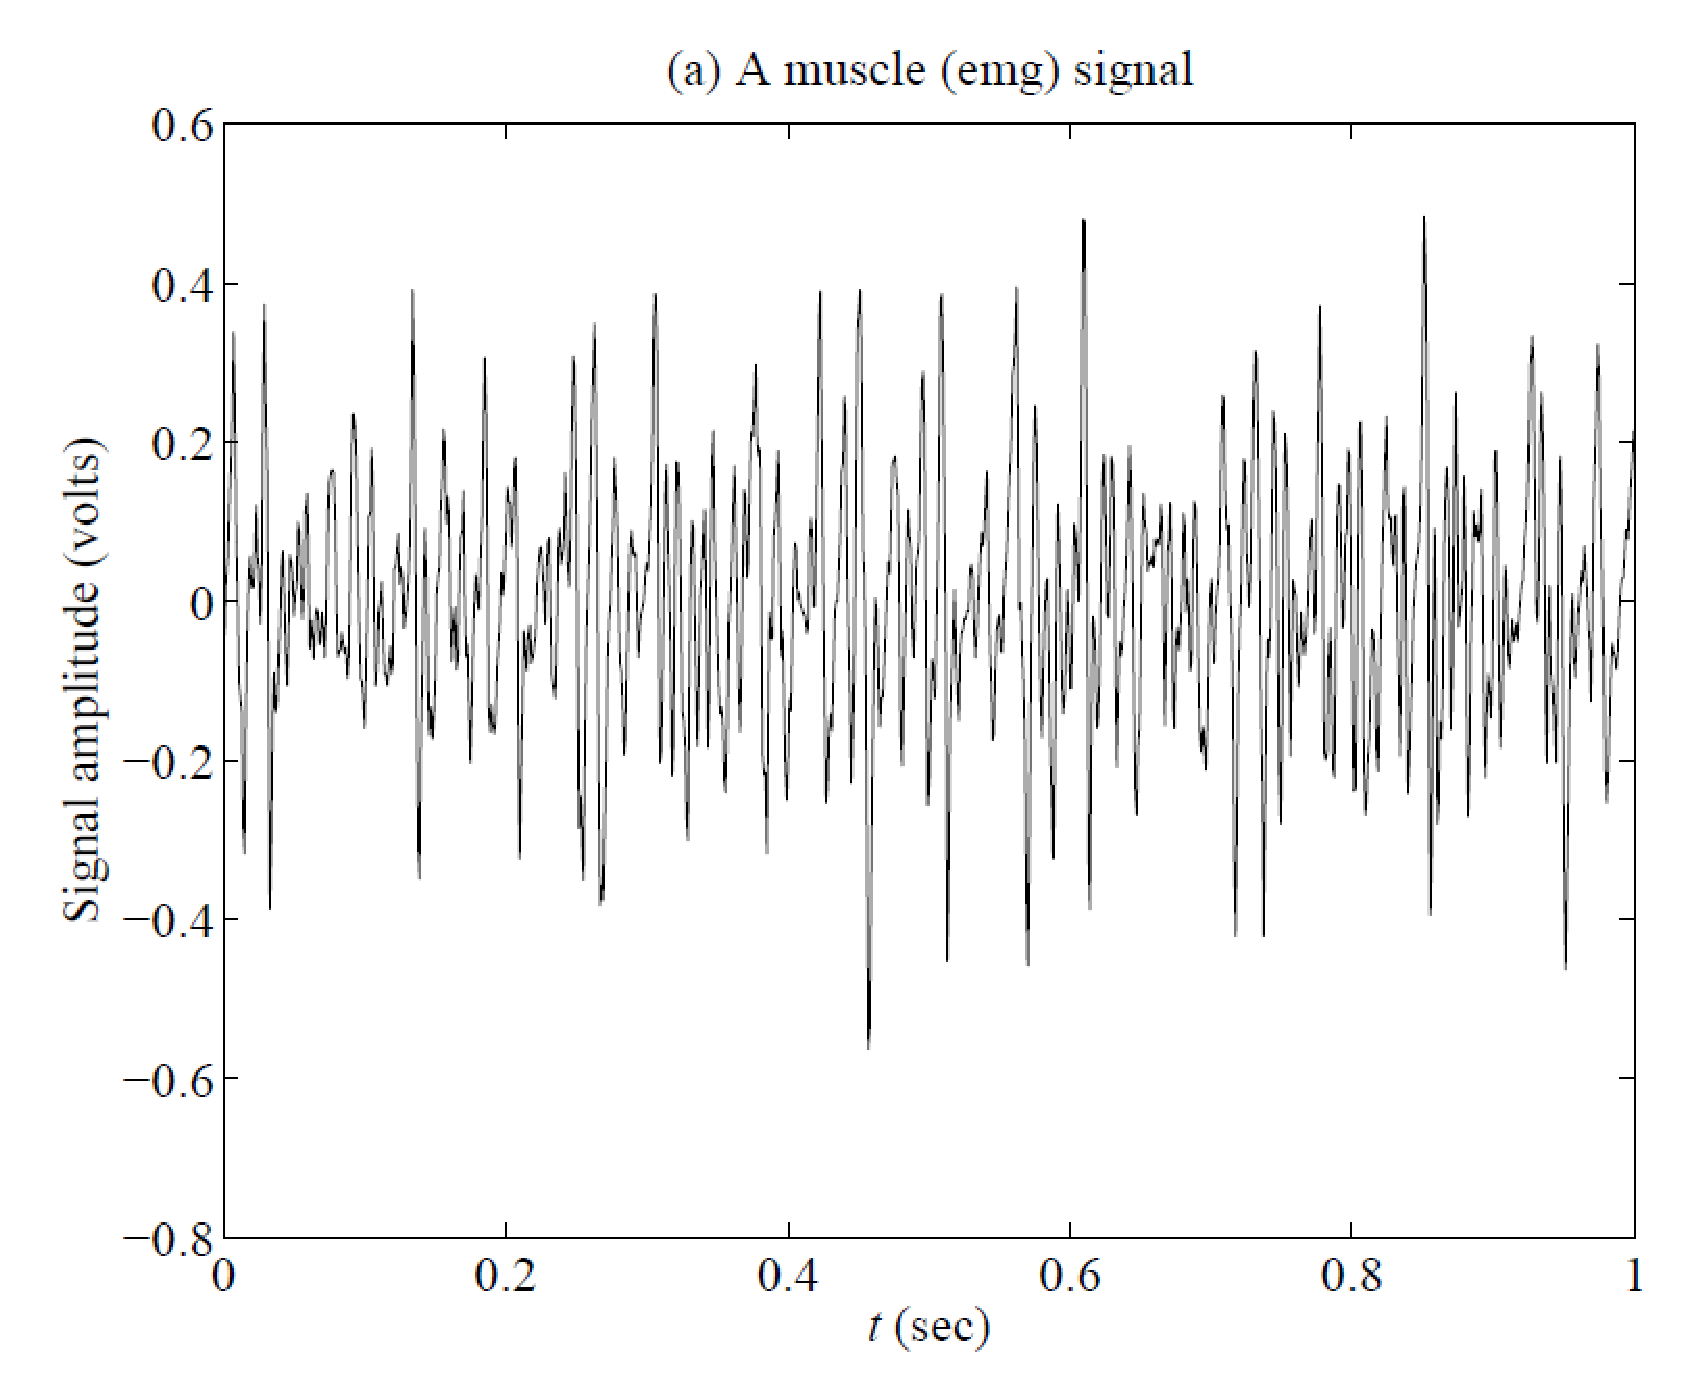
\includegraphics[width=0.77\columnwidth]{figs/fig14}
	  \end{center}
	\end{figure}
\end{frame}

\begin{frame}
    \frametitle{Variável Aleatória Gaussiana}

    \begin{figure}[t]
	  \begin{center}
	    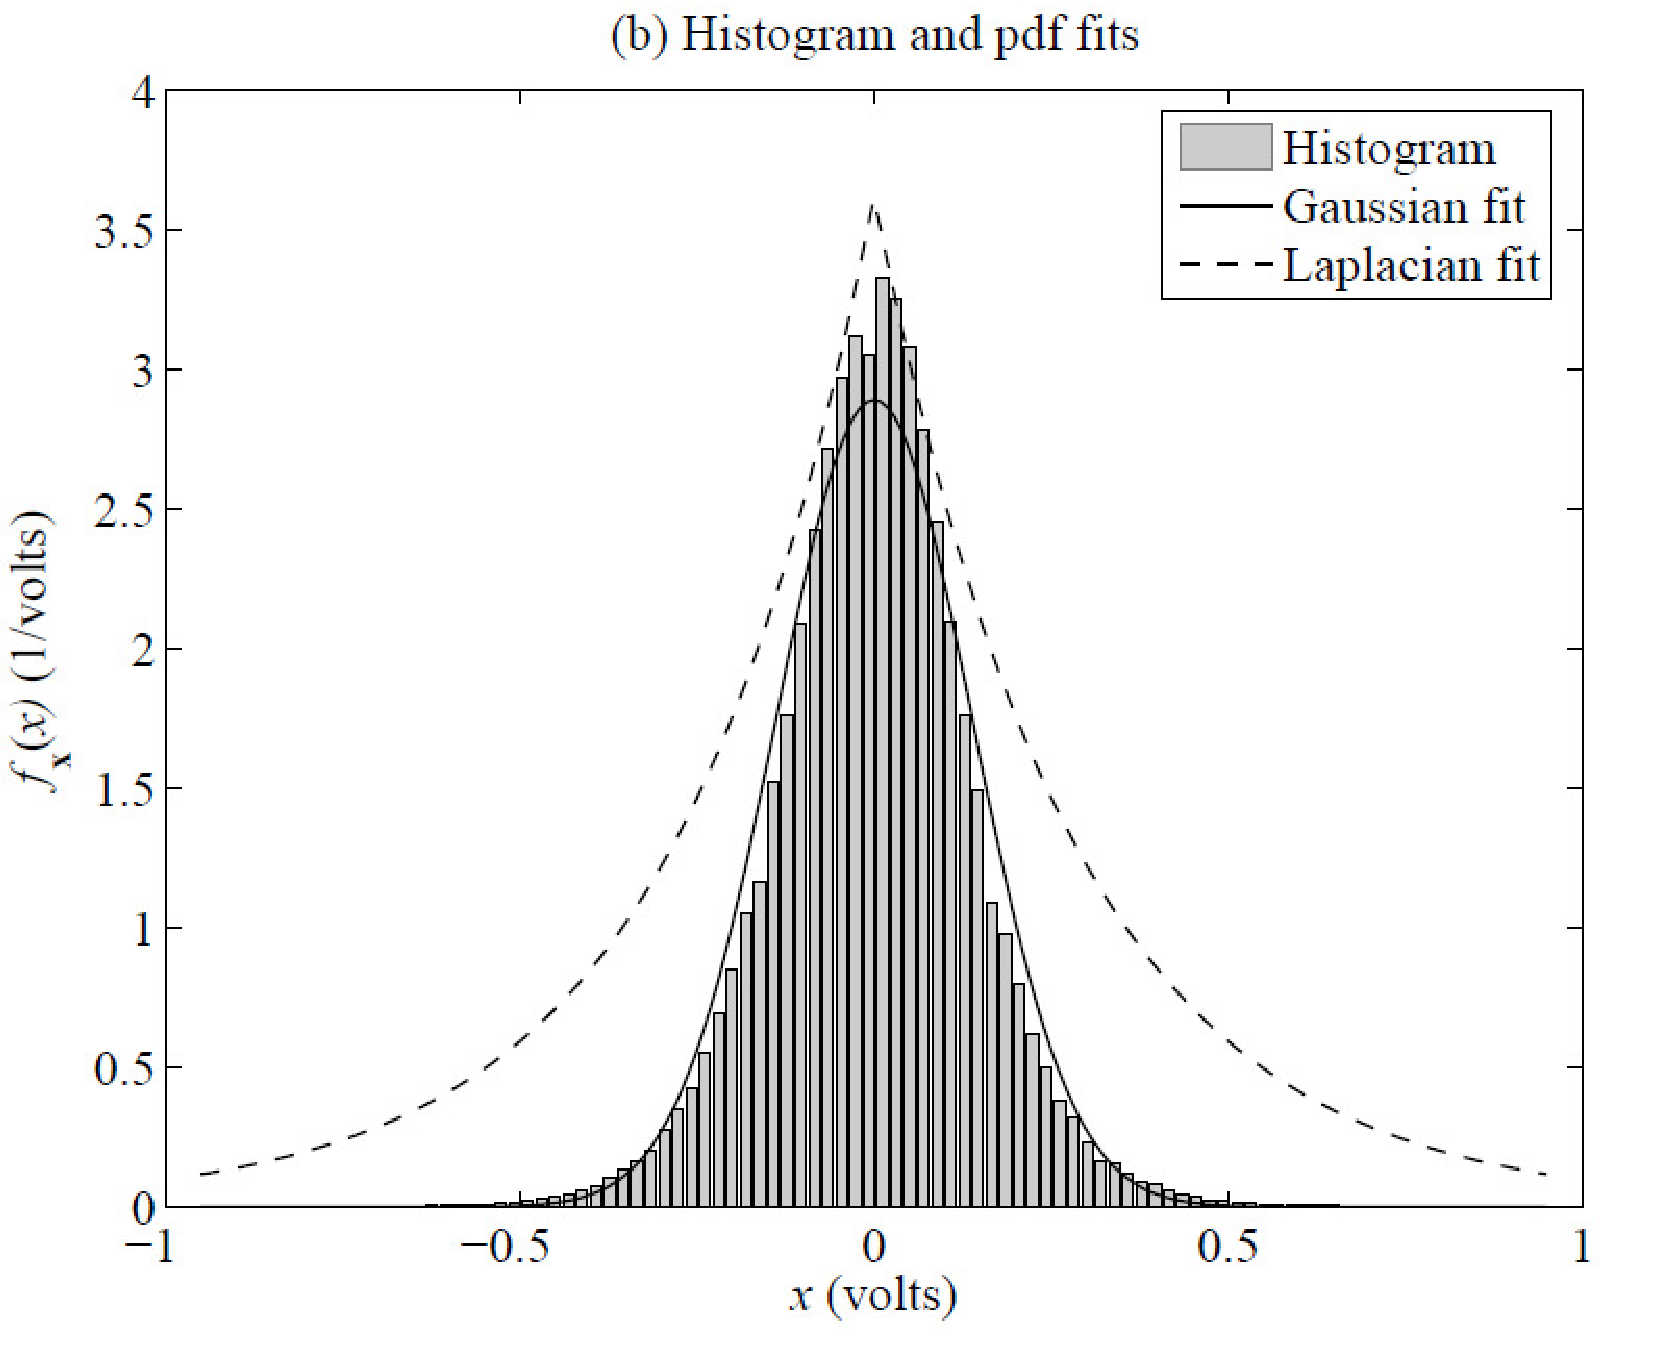
\includegraphics[width=0.77\columnwidth]{figs/fig15}
	  \end{center}
	\end{figure}
\end{frame}

\begin{frame}
    \frametitle{Funções de uma variável aleatória}

    \begin{itemize}
     \item A função $\mathbf{y} = g(\mathbf{x})$ é também uma variável aleatória.
      \item Pela definição, a CDF de $\mathbf{y}$ pode ser escrita como

      \begin{equation}
	  F_{\mathbf{y}}(y) = P(\omega \in \Omega \, | g(\mathbf{x}(\omega)) \leq y) \, ,
      \end{equation}

      \item Assuma que para todo $y$, a equação $g(x) = y$ possui um número de soluções finito e em cada ponto da solução, a derivada de $g(x)$ existe e é não-nula. A PDF de $\mathbf{y} = g(\mathbf{x})$ é dada por:

      \begin{equation}
	  f_{\mathbf{y}}(y) = \sum\limits_i \frac{f_{\mathbf{x}}(x_i)}{\left| \left. \frac{\mathrm{d}g(x)}{\mathrm{d}x} \right|_{x = x_i}  \right|} \, ,
      \end{equation}
      onde $\{x_i\}$ são as soluções de $g(x) = y$.
      \item Uma função linear de uma variável aleatória Gaussiana é também uma variável aleatória Gaussiana.

    \end{itemize}
   
\end{frame}

\begin{frame}
    \frametitle{Esperança de variáveis aleatórias - I}

    \begin{itemize}
     \item \textit{Médias estatísticas}, ou \textit{momentos}, possuem um papel importante na caracterização de uma variável aleatória.
     \item O \textit{valor esperado} (também chamado de valor médio ou primeiro momento) de uma variável aleatória $\mathbf{x}$ é definido como:

    \begin{equation}
	m_{\mathbf{x}} = E\{\mathbf{x}\} = \int_{-\infty}^{\infty} x f_{\mathbf{x}}(x) \mathrm{d}x \, ,
    \end{equation}
    onde $E$ denota o \textit{operador estatístico esperança}.
    \item Em geral, o n-ésimo momento de $\mathbf{x}$ é definido como:
    \begin{equation}
	E\{\mathbf{x}^n\} = \int_{-\infty}^{\infty} x^n f_{\mathbf{x}}(x) \mathrm{d}x \, .
    \end{equation}
    \item Para $n=2$, $E\{\mathbf{x}^2\}$ é conhecido como o valor médio quadrático da variável aleatória.
    \end{itemize}
   
\end{frame}

\begin{frame}
    \frametitle{Esperança de variáveis aleatórias - II}

    \begin{itemize}
     \item O n-ésimo \textit{momento central} da variável aleatória $\mathbf{x}$ é:

      \begin{equation}
	E\{\mathbf{y}\} = E\{(\mathbf{x} - m_{\mathbf{x}})^n\} = \int_{-\infty}^{\infty} (x-m_{\mathbf{x}})^n f_{\mathbf{x}}(x) \mathrm{d}x
      \end{equation}

      \item Quando $n=2$, o momento central é chamado de \textit{variância}, comumente denotado por $\sigma_{\mathbf{x}}^2$:

      \begin{equation}
	\sigma_{\mathbf{x}}^2 = \mathrm{var}(\mathbf{x}) = E\{(\mathbf{x} - m_{\mathbf{x}})^2\} = \int_{-\infty}^{\infty} (x-m_{\mathbf{x}})^2 f_{\mathbf{x}}(x) \mathrm{d}x
      \end{equation}
    
    \item A variância provê uma medida da ``aleatoriedade'' da variável.
    \item A média e variância de uma variável aleatória fornecem uma \textit{descrição parcial} de sua PDF.
    \item Relação entre a variância, o primeiro e o segundo momentos é dada por:
      \begin{equation}
	\sigma_{\mathbf{x}}^2 = E\{\mathbf{x}^2\} - [E\{\mathbf{x}\}]^2 = E\{\mathbf{x}^2\} - m_{\mathbf{x}}^2 \, .
      \end{equation}
    \end{itemize}
\end{frame}


\begin{frame}
    \frametitle{Variáveis aleatórias múltiplas - I}

    \begin{itemize}
     \item Normalmente encontradas quando tratando-se experimentos combinados ou tentativas repetidas de um único experimento.
      \item São basicamente funções multidimensionais definidas em um espaço amostral de um experimento combinado.
      \item Sejam $\mathbf{x}$ e $\mathbf{y}$ duas variáveis aleatórias definidas em um mesmo espaço amostral $\Omega$. A função distribuição de probabilidade conjunta é definida como:
      \begin{equation}
	  F_{\mathbf{x},\mathbf{y}} (x, y) = P(\mathbf{x} \leq x, \mathbf{y} \leq y)
      \end{equation}
      \item De forma análoga, a função densidade de probabilidade conjunta é dada por:
      \begin{equation}
	  f_{\mathbf{x},\mathbf{y}} (x, y) = \frac{\partial^2 F_{\mathbf{x},\mathbf{y}} (x, y)}{\partial x \partial y}
      \end{equation}
    
    \end{itemize}

\end{frame}

\begin{frame}
    \frametitle{Variáveis aleatórias múltiplas - II}

    \begin{itemize}
     \item Quando a PDF conjunta é integrada sobre uma das variáveis, uma obtém a PDF da outra variável, chamada de PDF marginal:
      \begin{align}
	  & \int_{-\infty}^{\infty} f_{\mathbf{x},\mathbf{y}} (x, y) \textrm{d}x = f_{\mathbf{y}}(y) \\
	  & \int_{-\infty}^{\infty} f_{\mathbf{x},\mathbf{y}} (x, y) \textrm{d}y = f_{\mathbf{x}}(x)
      \end{align}
      \item Note que:
      \begin{align}
	  & \int_{-\infty}^{\infty}\int_{-\infty}^{\infty} f_{\mathbf{x},\mathbf{y}} (x, y) \textrm{d}x\textrm{d}y = F(\infty, \infty) = 1 \\
	  & F_{\mathbf{x},\mathbf{y}}(-\infty,-\infty) = F_{\mathbf{x},\mathbf{y}}(-\infty,y) = F_{\mathbf{x},\mathbf{y}}(x,-\infty) = 0
      \end{align}
    
    \end{itemize}

\end{frame}

\begin{frame}
    \frametitle{Variáveis aleatórias múltiplas - III}

    \begin{itemize}
     \item A PDF condicional da variável aleatória $\mathbf{y}$, dado que o valor da variável aleatória $\mathbf{x}$ é igual a $x$, é definida como:
      \begin{equation}
      f_{\mathbf{y}}(y|x) =  \begin{cases}
				    \frac{f_{\mathbf{x},\mathbf{y}}(x,y)}{f_{\mathbf{x}}(x)} \, , & f_{\mathbf{x}}(x) \neq 0 \\
				    0 \, , & \mathrm{c.c.}
                               \end{cases}
      \end{equation}
      \item Duas variáveis aleatórias $\vax$ e $\vay$ são estatísticamente independentes se e somente se:
      \begin{align}
	  & f_{\vay}(y|x) = f_{\vay}(y) \qquad \textrm{ou de forma equivalente} \\
	  & f_{\vax,\vay}(x,y) = f_{\vax}(x)f_{\vay}(y)
      \end{align}
      \item O \textit{momento conjunto} é definido como:
      \begin{equation}
	  E\{\vax^j\vay^k\} = \int_{-\infty}^{\infty}\int_{-\infty}^{\infty} x^j y^k f_{\vax,\vay}(x,y)\mathrm{d}x\mathrm{d}y \, .
      \end{equation}
      
    \end{itemize}

\end{frame}

\begin{frame}
    \frametitle{Variáveis aleatórias múltiplas - IV}

    \begin{itemize}
     \item O \textit{momento central conjunto} é:
      \begin{equation}
	  E\{(\vax-m_{\vax})^j(\vay-m_{\vay})^k\} = \int_{-\infty}^{\infty}\int_{-\infty}^{\infty} (x-m_{\vax})^j (y-m_{\vay})^k f_{\vax,\vay}(x,y)\mathrm{d}x\mathrm{d}y \, ,
      \end{equation}
      onde $m_{\vax} = E\{\vax\}$ e $m_{\vay} = E\{\vay\}$.
      \item Os momentos mais importantes são:
      \begin{itemize}
       \item Correlação:
	\begin{equation}
	    E\{\vax\vay\} = \int_{-\infty}^{\infty}\int_{-\infty}^{\infty} x y f_{\vax,\vay}(x,y)\mathrm{d}x\mathrm{d}y
	\end{equation}
	\item Covariância:
	\begin{equation}
	    \mathrm{cov}\{\vax,\vay\} = E\{(\vax-m_{\vax})(\vay-m_{\vay})\} = E\{\vax\vay\} - m_{\vax}m_{\vay}
	\end{equation}

      \end{itemize}

    \end{itemize}
    
\end{frame}

\begin{frame}
    \frametitle{Variáveis aleatórias múltiplas - V}

    \begin{itemize}
     \item Sejam $\sigma_{\vax}^2$ e $\sigma_{\vay}^2$ as variâncias de $\vax$ e $\vay$, respectivamente. A covariância normalizada com relação a $\sigma_{\vax}\sigma_{\vay}$ é chamada de \textit{coeficiente de correlação}:
      \begin{equation}
	  \rho_{\vax,\vay} = \frac{\mathrm{cov}\{\vax,\vay\}}{\sigma_{\vax}\sigma_{\vay}} \, .
      \end{equation}
    \item $\rho_{\vax,\vay}$ indica o grau de \textit{dependência linear} entre duas variáveis aleatórias. 
    \item Pode-se mostrar que $|\rho_{\vax,\vay}| \leq 1$.
    \item Se $\rho_{\vax,\vay} = 0$, $\vax$ e $\vay$ são ditas \textit{descorrelacionadas}.
    \item Pode-se verificar que se $\vax$ e $\vay$ são independentes, então $\rho_{\vax,\vay} = 0$: \textit{independência implica em ausência de correlação}.
    \item No entanto, ausência de correlação não necessariamente implica em independência estatística.
    \end{itemize}
    
\end{frame}

\begin{frame}
    \frametitle{Processos aleatórios - I}

    \begin{figure}[t]
	  \begin{center}
	    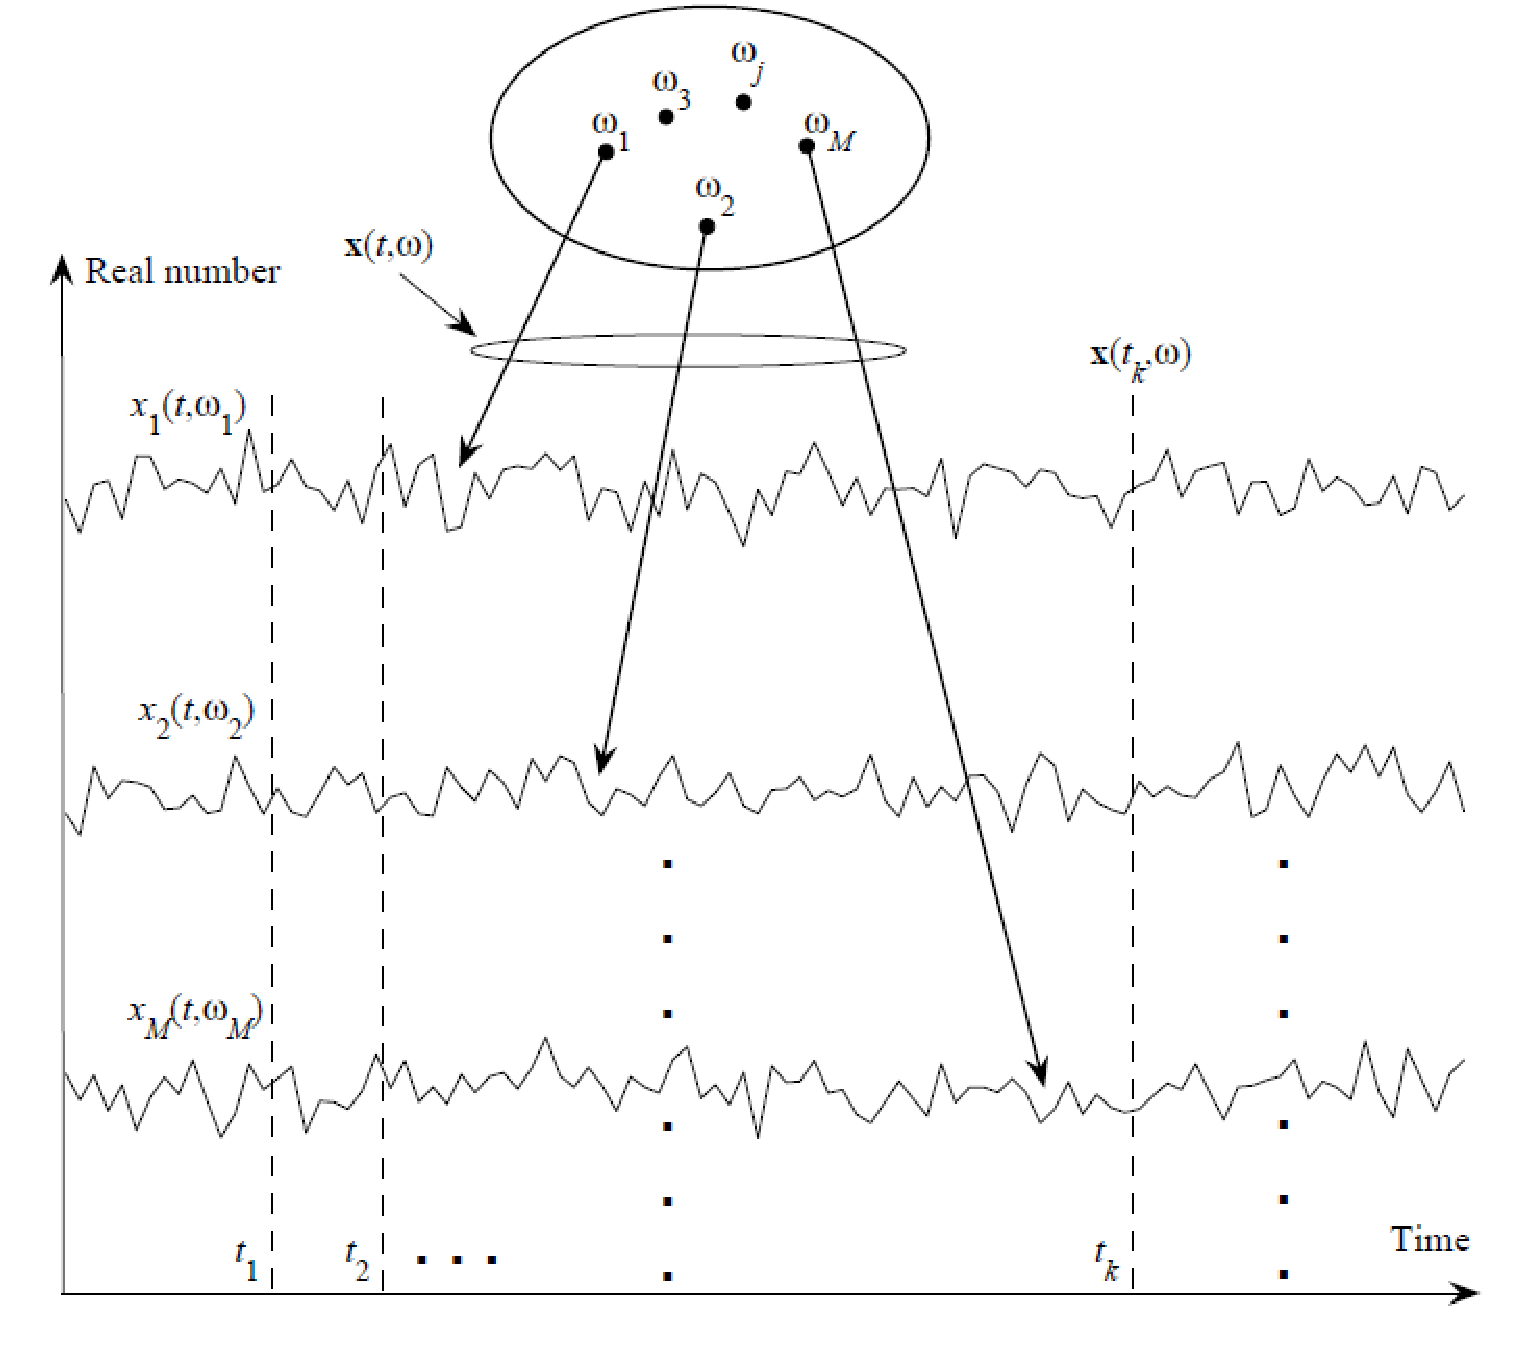
\includegraphics[width=0.5\columnwidth]{figs/fig22}
	  \end{center}
	\end{figure}
     Mapeamento de um espaço amostral em um \textit{conjunto de funções temporais}. 
\end{frame}

\begin{frame}
    \frametitle{Processos aleatórios - II}

    \begin{itemize}
     \item \textit{Ensemble}: conjunto de possíveis funções temporais denotado por $\vax(t)$, onde as funções temporais $x_1(t,\omega_1), x_2(t,\omega_2), x_3(t,\omega_3), \ldots$, são membros específicos do ensemble.
      \item Em um dado instante $t=t_k$, temos a variável aleatória $\vax(t_k)$.
      \item Em quaisquer dois instantes de tempo $t_1$ e $t_2$, temos duas diferentes variáveis aleatórias $\vax(t_1)$ e $\vax(t_2)$. Qualquer relação entre elas é descrita pela PDF conjunta $f_{\vax(t_1),\vax(t_2)}(x_1,x_2;t_1,t_2)$.
      \item Descrição completa do processo aleatório é determinada pela PDF conjunta $f_{\vax(t_1),\vax(t_2),\ldots,\vax(t_N)}(x_1,x_2,\ldots,x_N;t_1,t_2,\ldots,t_N)$.
      \item PDFs conjuntas mais importantes:
      \begin{itemize}
       \item Primeira ordem: $f_{\vax(t)}(x;t)$
	\item Segunda ordem: $f_{\vax(t_1),\vax(t_2)}(x_1,x_2;t_1,t_2)$
      \end{itemize}

    \end{itemize}

\end{frame}

\begin{frame}
    \frametitle{Exemplos de processos aleatórios - I}

    \begin{figure}[t]
	  \begin{center}
	    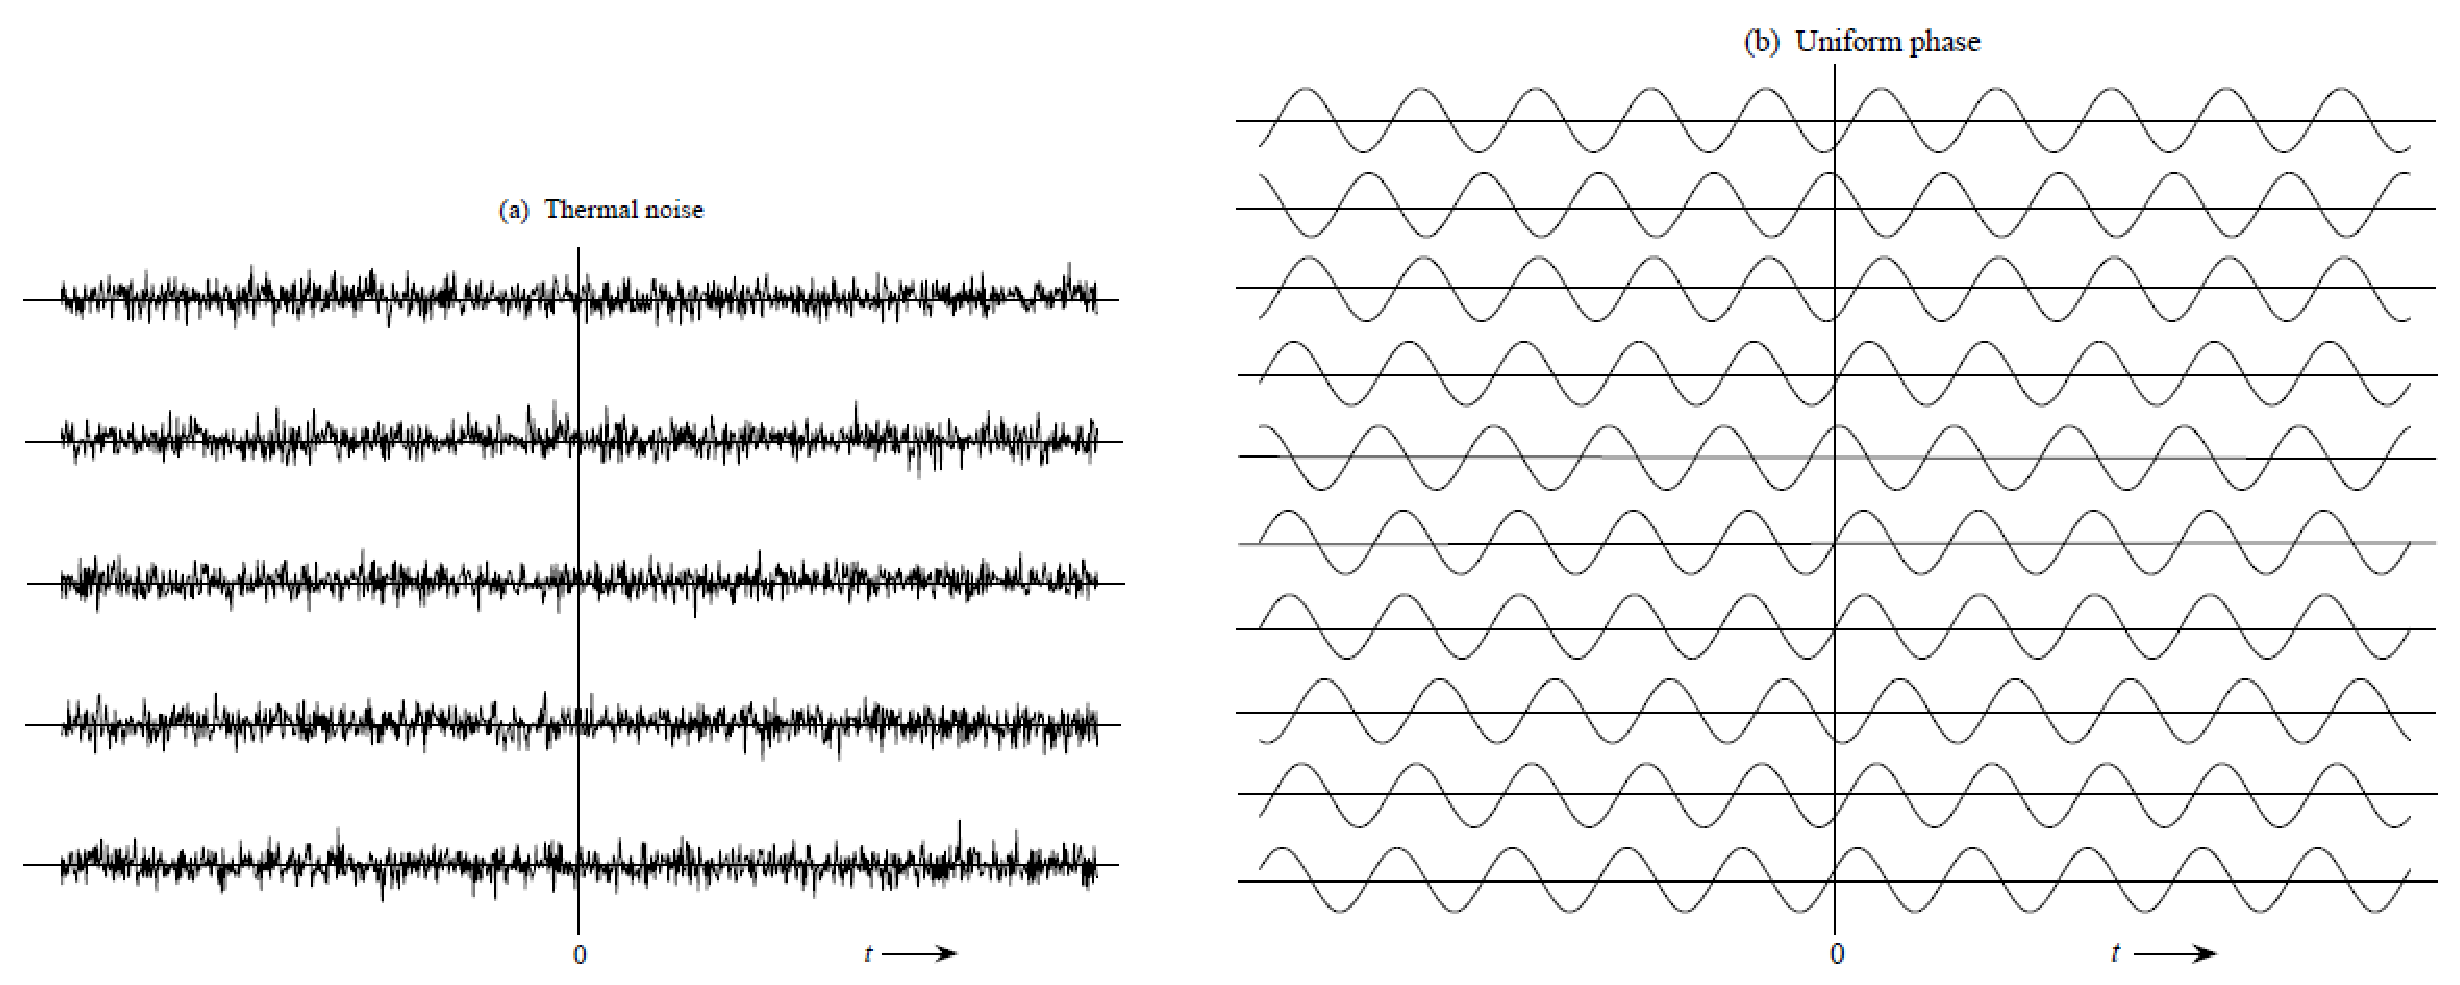
\includegraphics[width=0.95\columnwidth]{figs/fig23}
	  \end{center}
	\end{figure}
     
\end{frame}

\begin{frame}
    \frametitle{Exemplos de processos aleatórios - II}

    \begin{figure}[t]
	  \begin{center}
	    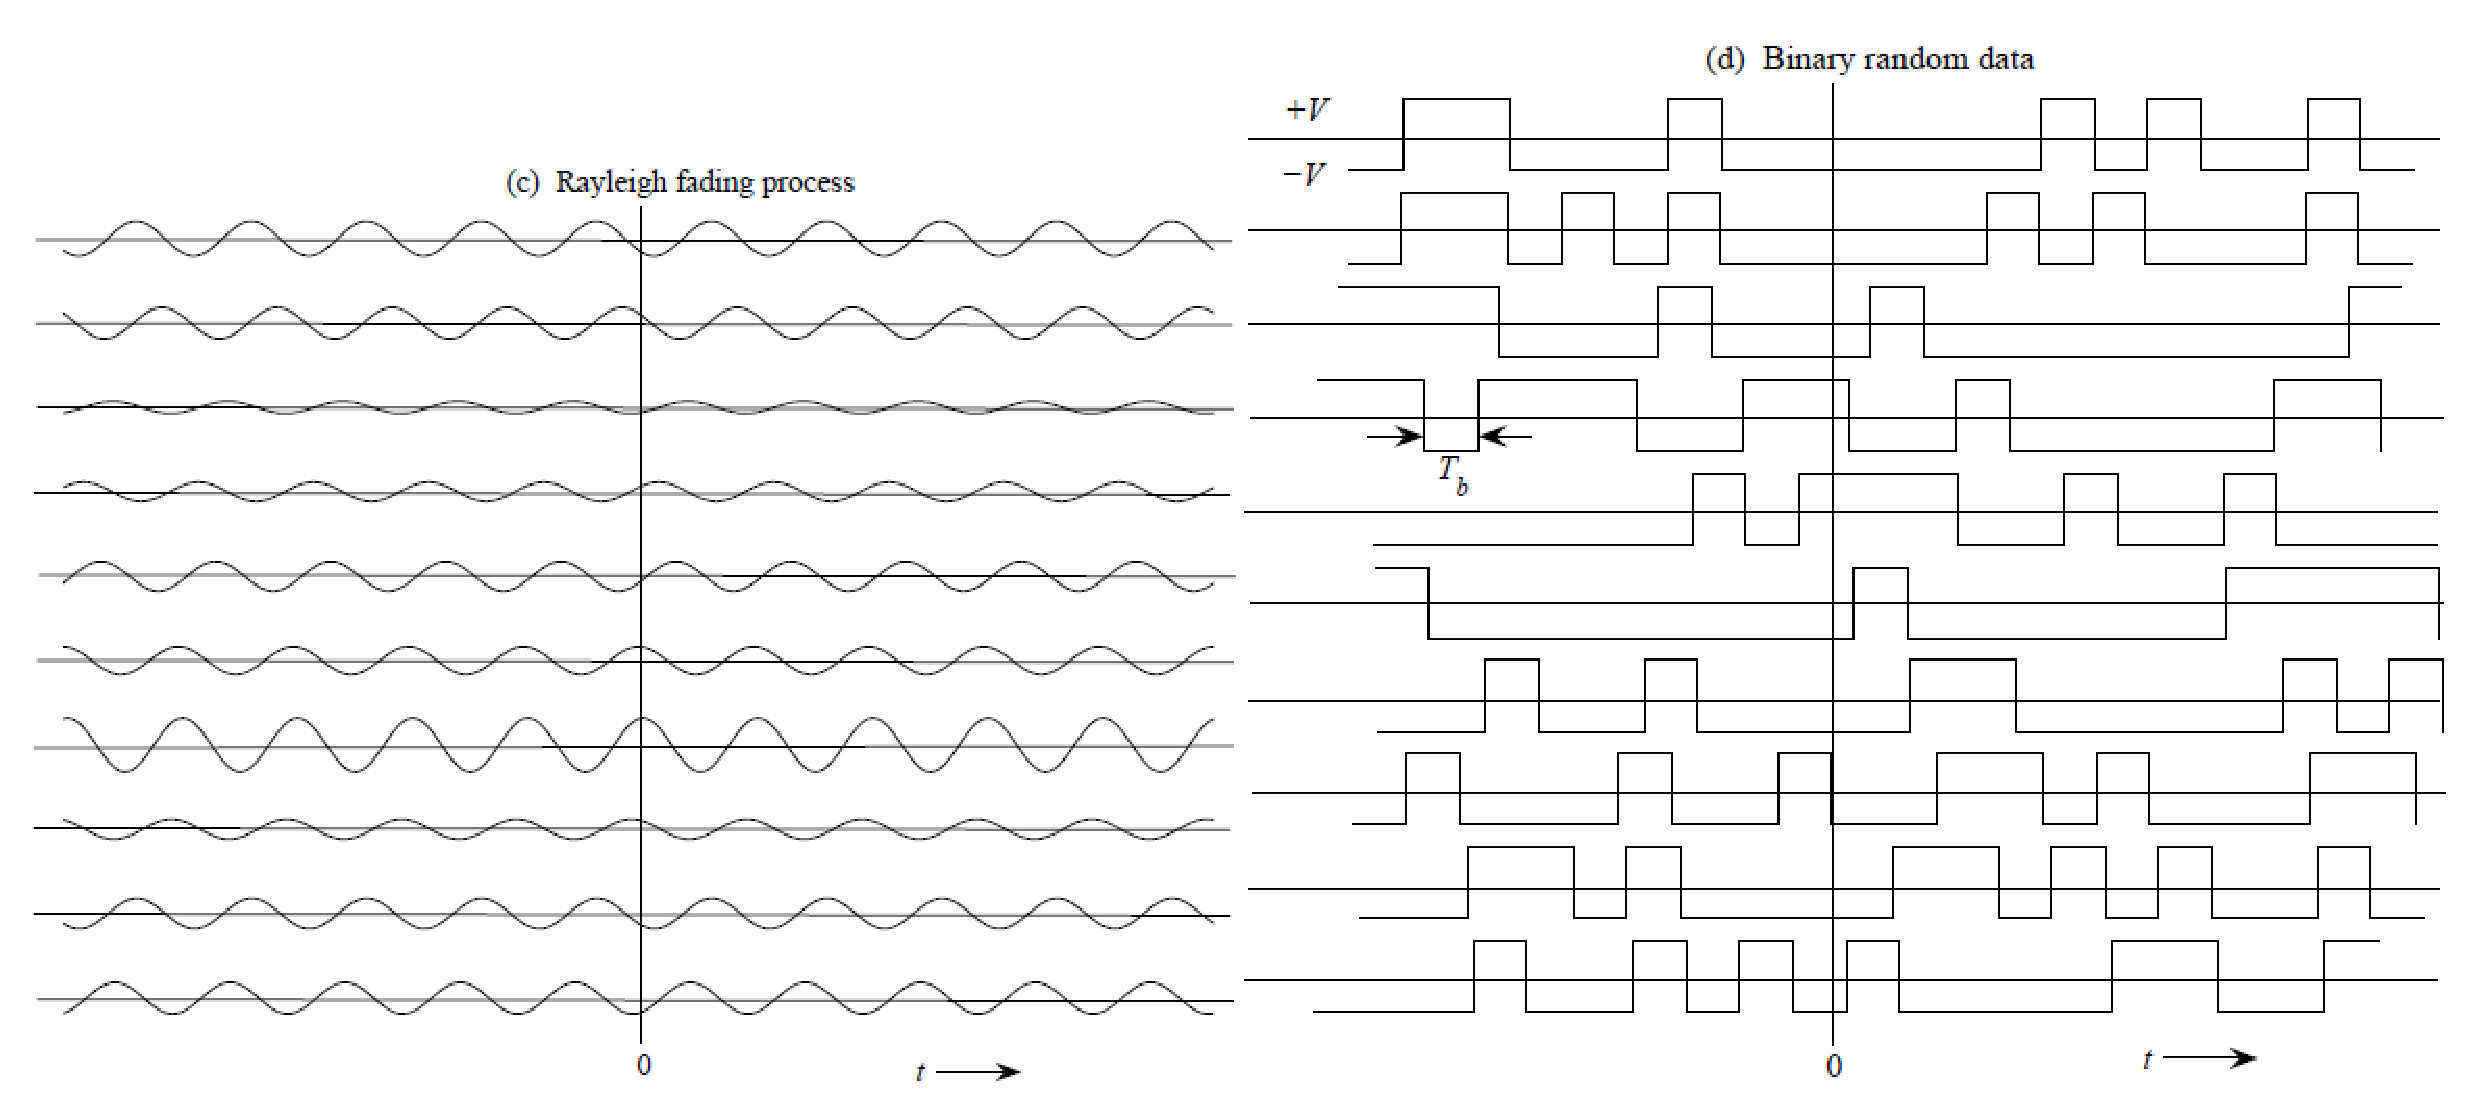
\includegraphics[width=0.95\columnwidth]{figs/fig24}
	  \end{center}
	\end{figure}
     
\end{frame}

\begin{frame}
    \frametitle{Classificação de processos aleatórios}

    \begin{itemize}
     \item Baseada na mudança das estatísticas com o tempo o processo pode ser: \textit{não-estacionário} ou \textit{estacionário}.
      \item Diferentes níveis de estacionariedade:
      \begin{itemize}
       \item Estritamente estacionário: a PDF conjunta de qualquer ordem é independente de um deslocamento temporal.
	\item Estacionariedade de ordem $N$: a PDF conjunta não depende do deslocamento temporal, mas depende de espaçamentos no tempo:
	\begin{align*}
	  f_{\vax(t_1),\vax(t_2),\ldots,\vax(t_N)}&(x_1,x_2,\ldots,x_n; t_1,t_2,\ldots,t_N) = \\
	  f_{\vax(t_1+t),\vax(t_2+t),\ldots,\vax(t_N+t)}&(x_1,x_2,\ldots,x_n; t_1+t,t_2+t,\ldots,t_N+t)
	\end{align*}
	\item Estacionariedade de primeira ordem:
	\begin{equation}
	  f_{\vax(t_1)}(x; t_1) = f_{\vax(t_1+t)}(x; t_1+t) = f_{\vax(t)}(x)
	\end{equation}
	\item Estacionariedade de segunda ordem:
	\begin{align*}
	  f_{\vax(t_1),\vax(t_2)}(x_1,x_2; t_1,t_2) &= f_{\vax(t_1+t),\vax(t_2+t)}(x_1,x_2; t_1+t, t_2+t) \\
	  &= f_{\vax(t_1),\vax(t_2)}(x_1,x_2; \tau), \qquad \tau = t_2 - t_1 \, .
	\end{align*}

      \end{itemize}

    \end{itemize}
     
\end{frame}

\begin{frame}
    \frametitle{Médias estatísticas ou momentos conjuntos}

    \begin{itemize}
     \item Considere $N$ variáveis aleatórias $\vax(t_1),\vax(t_2),\ldots,\vax(t_N)$. Os momentos conjuntos destas variáveis aleatórias são dados por:
    \begin{align*}
	E\{\vax^{k_1}(t_1),&\vax^{k_2}(t_2),\ldots,\vax^{k_N}(t_N)\} = \int_{x_1=-\infty}^{\infty} \cdots \int_{x_N=-\infty}^{\infty} \\
	&x_1^{k_1}x_2^{k_2} \cdots x_N^{k_N} f_{\vax(t_1),\vax(t_2),\ldots,\vax(t_N)}(x_1,x_2,\ldots,x_N; t_1,t_2,\ldots,t_N) \\
	& \mathrm{d}x_1 \mathrm{d}x_2 \ldots \mathrm{d}x_N \, ,
    \end{align*}

      para todos os inteiros $k_j \geq 1$ e $N \geq 1$.
      
      \item Vamos considerar somente os momentos de primeira e segunda ordem, i.e., $E\{\vax(t)\}$ (média), $E\{\vax^2(t)\}$ (valor quadrático médio) e $E\{\vax(t_1)\vax(t_2)\}$ (autocorrelação).
    \end{itemize}
     
\end{frame}

\begin{frame}
    \frametitle{Valor médio ou primeiro momento}

    \begin{itemize}
     \item O valor médio do processo em um tempo $t$ é:
      \begin{equation}
	  m_{\vax}(t) = E\{\vax(t)\} = \int_{-\infty}^{\infty} x f_{\vax(t)} (x;t) \mathrm{d}x \, .
      \end{equation}
      \item A média se dá ao longo do ensemble, e se a PDF varia com o tempo então o valor médio é uma função determinística do tempo.
      \item Se um processo é estacionário então a média é independente de $t$ ou uma constante.
\	\begin{equation}
 	 m_{\vax} = E\{\vax(t)\} = \int_{-\infty}^{\infty}x f_{\vax}(x) \mathrm{d}x \, . 
 	\end{equation}

    \end{itemize}
     
\end{frame}

\begin{frame}
    \frametitle{Valor quadrático médio ou segundo momento}

    \begin{itemize}
     \item O valor quadrático médio (MSV) é definido como:
      \begin{align*}
	  \mathrm{MSV}_{\vax}(t) &= E\{\vax^2(t)\} = \int_{-\infty}^{\infty} x^2 f_{\vax(t)}(x;t)\mathrm{d}x \quad &\textrm{(não-estac.)} \\
	  \mathrm{MSV}_{\vax} &= E\{\vax^2(t)\} = \int_{-\infty}^{\infty} x^2 f_{\vax}(x)\mathrm{d}x \quad &\textrm{(estac.)}
      \end{align*}
      \item O segundo momento central (ou variância) é:
      \begin{align*}
	  \sigma_{\vax}^2(t) &= E\{[\vax(t) - m_{\vax}(t)]^2\} = \mathrm{MSV}_{\vax}(t)  - m_{\vax}^2(t) \quad &\textrm{(não-estac.)} \\
	  \sigma_{\vax}^2 &= E\{[\vax(t) - m_{\vax}]^2\} = \mathrm{MSV}_{\vax}  - m_{\vax}^2 \quad &\textrm{(estac.)}
      \end{align*}

    \end{itemize}
     
\end{frame}

\begin{frame}
    \frametitle{Correlação}

    \begin{itemize}
     \item A função de autocorrelação descreve completamente a densidade espectral de potência do processo aleatório.
      \item Pode ser definida como a correlação entre duas variáveis aleatórias $\vax_1 = \vax(t_1)$ e $\vax_2 = \vax(t_2)$:
      \begin{small}
      \begin{align*}
	  R_{\vax}(t_1,t_2) = E\{\vax(t_1)\vax(t_2)\} = \int_{x_1=-\infty}^{\infty}\int_{x_2=-\infty}^{\infty} x_1 x_2 f_{\vax_1,\vax_2}(x_1,x_2;t_1,t_2)\mathrm{d}x_1\mathrm{d}x_2
      \end{align*}\end{small}
      \item Para um processo estacionário:
      \begin{small}
      \begin{align*}
	  R_{\vax}(\tau) = E\{\vax(t)\vax(t+\tau)\} = \int_{x_1=-\infty}^{\infty}\int_{x_2=-\infty}^{\infty} x_1 x_2 f_{\vax_1,\vax_2}(x_1,x_2;\tau)\mathrm{d}x_1\mathrm{d}x_2
      \end{align*}\end{small}
      \item Processo com \textit{estacionariedade no sentido amplo} (WSS): 
      \begin{itemize}
       \item $E\{\vax(t)\} = m_{\vax}$ para qualquer $t$, e $R_{\vax}(t_1,t_2) = R_{\vax}(\tau)$ para $\tau = t_2 - t_1$.
      \end{itemize}

    \end{itemize}
     
\end{frame}

\begin{frame}
    \frametitle{Propriedades da autocorrelação de um processo WSS}

    \begin{itemize}
     \item $R_{\vax}(\tau) = R_{\vax}(-\tau)$. É uma função par de $\tau$, uma vez que o mesmo conjunto de valores é mediado ao longo do ensemble, independente da direção de translação.
      \item $|R_{\vax}(\tau)| \leq R_{\vax}(0)$. O valor máximo sempre ocorre em $\tau = 0$. Além disso, $R_{\vax}(0)$ é o valor médio quadrático do processo aleatório.
      \item Se para um certo $\tau_0$ temos que $R_{\vax}(\tau_0) = R_{\vax}(0)$, então para qualquer inteiro $k$, $R_{\vax}(k\tau_0) = R_{\vax}(0)$.
      \item Se $m_{\vax} \neq 0$ então $R_{\vax}(\tau)$ possuirá uma componente constante igual a $m_{\vax}^2$.
      \item Funções de autocorrelação não podem ter uma forma arbitrária. A restrição da forma surge do fato de que a transformada de Fourier de uma função de autocorrelação deve ser maior ou igual a zero, i.e., $\mathcal{F}\{R_{\vax}(\tau)\} \geq 0$.
    \end{itemize}
     
\end{frame}

\begin{frame}
    \frametitle{Densidade espectral de potência de um processo aleatório - I}

    \begin{itemize}
     \item Um processo aleatório é um sinal de energia infinita, portanto não se pode tirar diretamente sua transformada de Fourier.
      \begin{figure}[t]
	  \begin{center}
	    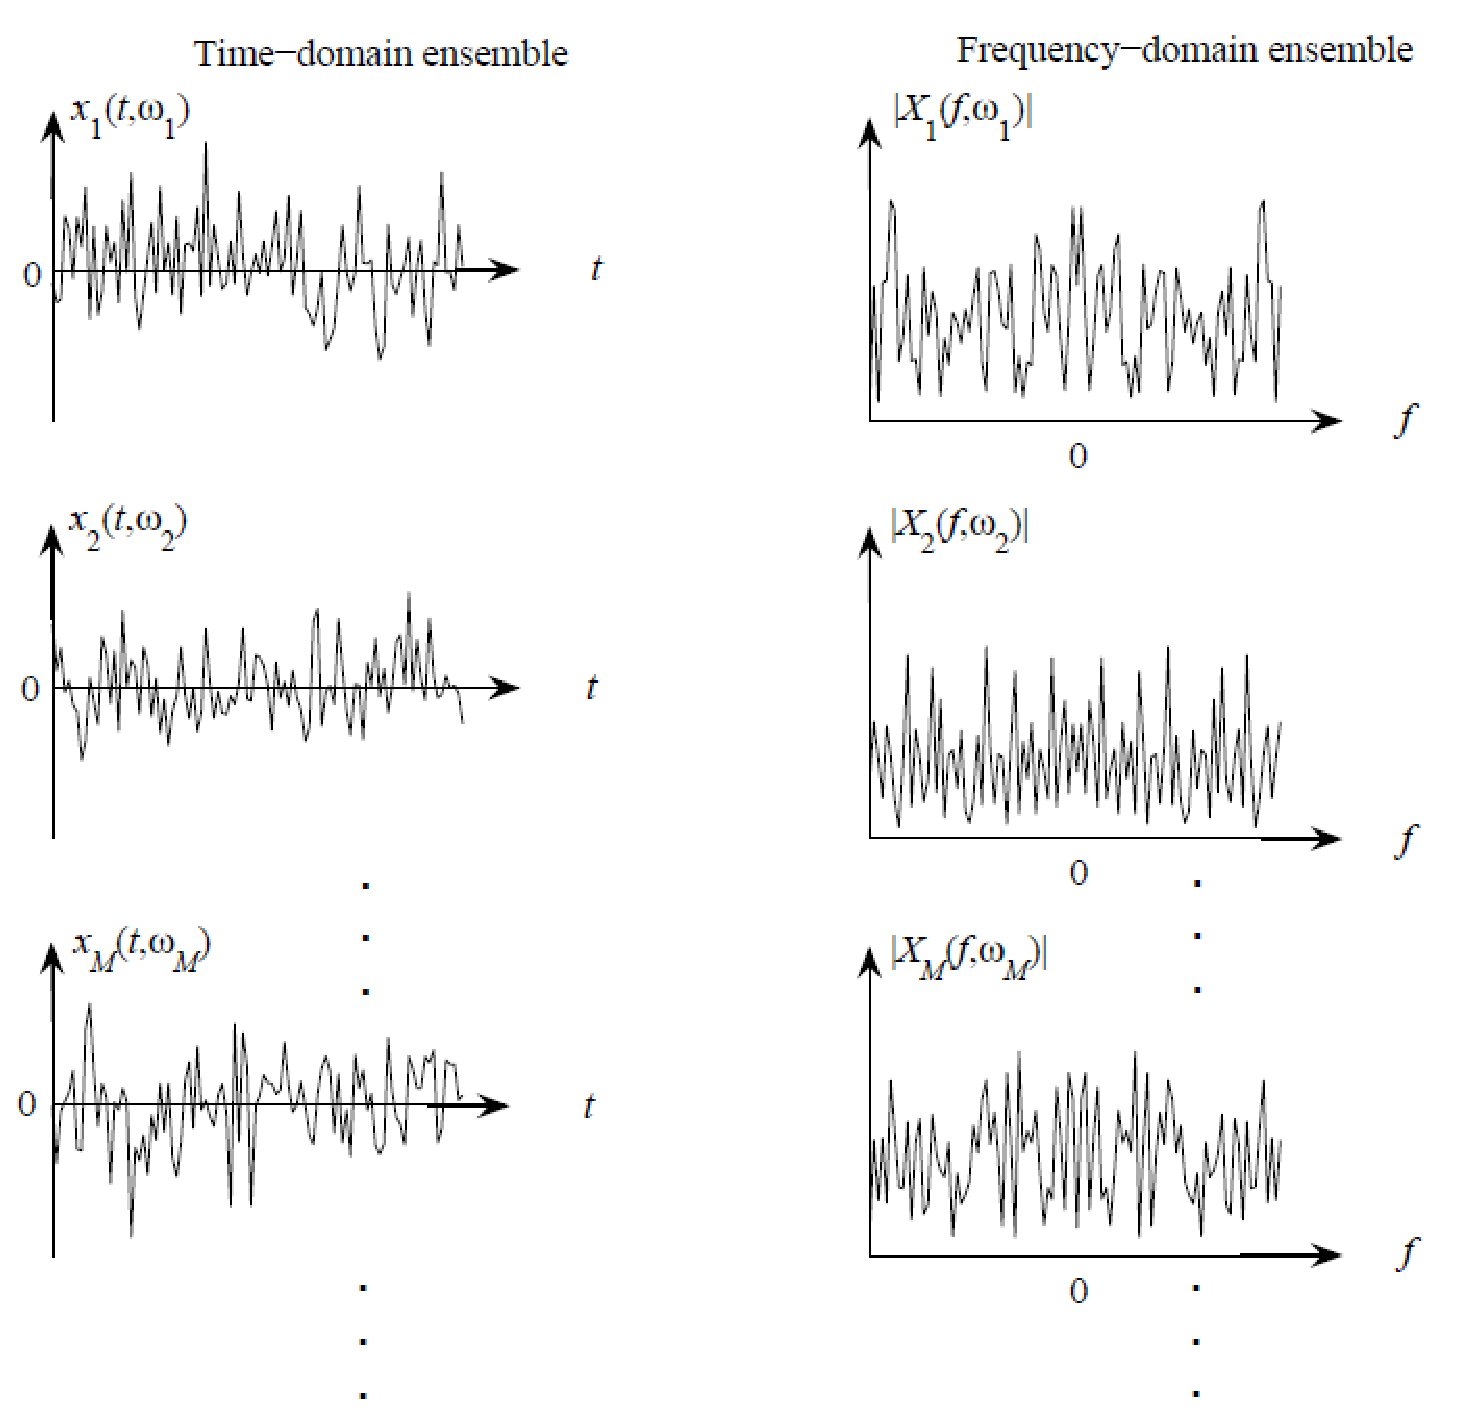
\includegraphics[width=0.55\columnwidth]{figs/fig25}
	  \end{center}
	\end{figure}
    \end{itemize}
     
\end{frame}

\begin{frame}
    \frametitle{Densidade espectral de potência de um processo aleatório - II}

    \begin{itemize}
     \item É necessário determinar como a potência média do processo se distribui na freqüência.
      \item Defina um processo truncado:

      \begin{equation}
	  \vax_T(t) = \begin{cases} \vax(t), \quad &-T \leq t \leq T \\ 0, \quad &\mathrm{c.c.} \end{cases} 
      \end{equation}
      \item Considere a transformada de Fourier do processo truncado:
      \begin{equation}
	  \mathbf{X}_T(f) = \int_{-\infty}^{\infty} \vax_T(t) \mathrm{e}^{-j2\pi ft} \mathrm{d}t \, .
      \end{equation}
      \item Medie a energia sobre o tempo total, $2T$:
      \begin{equation}
	  \mathbf{P} = \frac{1}{2T} \int_{-T}^T \vax_T^2(t)\mathrm{d}t = \frac{1}{2T} \int_{-\infty}^{\infty} |\mathbf{X}_T(f)|^2 \mathrm{d}f \quad \mathrm{(Watts)}
      \end{equation}

    \end{itemize}
          
\end{frame}

\begin{frame}
    \frametitle{Densidade espectral de potência de um processo aleatório - III}

    \begin{itemize}
     \item Encontre o valor médio de $\mathbf{P}$:
      \begin{equation}
	  E\{\mathbf{P}\} = E\left\{\frac{1}{2T} \int_{-T}^T \vax_T^2(t) \mathrm{d}t \right\} = E\left\{\frac{1}{2T} \int_{-\infty}^{\infty} |\mathbf{X}_T(f)|^2 \mathrm{d}f \right\}
      \end{equation}
      \item Toma-se o limite quando o período tende a infinito:
      \begin{equation}
	  \lim_{T \rightarrow \infty} \frac{1}{2T} \int_{-T}^T E\{\vax_T^2(t)\} \mathrm{d}t = \lim_{T \rightarrow \infty} \frac{1}{2T} \int_{-\infty}^{\infty} E\left\{ |\mathbf{X}_T(f)|^2 \right\} \mathrm{d}f \, .
      \end{equation}
      \item Segue que:
      \begin{equation}
	  \mathrm{MSV}_{\vax} = \int_{-\infty}^{\infty} \lim_{T \rightarrow \infty} \frac{E\left\{ |\mathbf{X}_T(f)|^2 \right\}}{2T}  \mathrm{d}f \quad \mathrm{(Watts)}
      \end{equation}

    \end{itemize}
          
\end{frame}

\begin{frame}
    \frametitle{Densidade espectral de potência de um processo aleatório - IV}

    \begin{itemize}
     \item Finalmente a \textit{densidade espectral de potência} é dada por:
      \begin{equation}
	  S_{\vax}(f) = \lim_{T \rightarrow \infty}\frac{E\left\{ |\mathbf{X}_T(f)|^2 \right\}}{2T} \quad \mathrm{(Watts/Hz)}
      \end{equation}
      \item Pode-se mostrar que a densidade espectral de potência e a função de autocorrelação formam um \textit{par da transformada de Fourier}:
      \begin{equation}
	  R_{\vax}(\tau) \longleftrightarrow S_{\vax}(f) = \int_{\tau = -\infty}^{\infty} R_{\vax}(\tau)\mathrm{e}^{-j2\pi f\tau}\mathrm{d}\tau \,.
      \end{equation}

    \end{itemize}
          
\end{frame}
 
\begin{frame}
    \frametitle{Média temporal e ergodicidade}

    \begin{itemize}
     \item Um processo é \textit{ergódico} quando qualquer membro do ensemble exibe o mesmo comportamento estatístico que todo o ensemble.
      \item Todas as médias temporais em um dado membro do ensemble são iguais à correspondente média do ensemble:
      \begin{equation}
	  E\{\vax^n (t) \} = \int_{-\infty}^{\infty} x^n f_{\vax}(x)\mathrm{d}x
      \end{equation}
      \item Em um processo ergódico: para medir diversas médias estatísticas, basta olhar para uma única realização do processo e encontrar a média temporal correspondente.
      \item Para um processo ser ergódico ele tem que ser estacionário. O reverso não é verdadeiro.

    \end{itemize}
          
\end{frame}

\begin{frame}
    \frametitle{Processos aleatórios e sistemas LTI}

    \begin{figure}[t]
	  \begin{center}
	    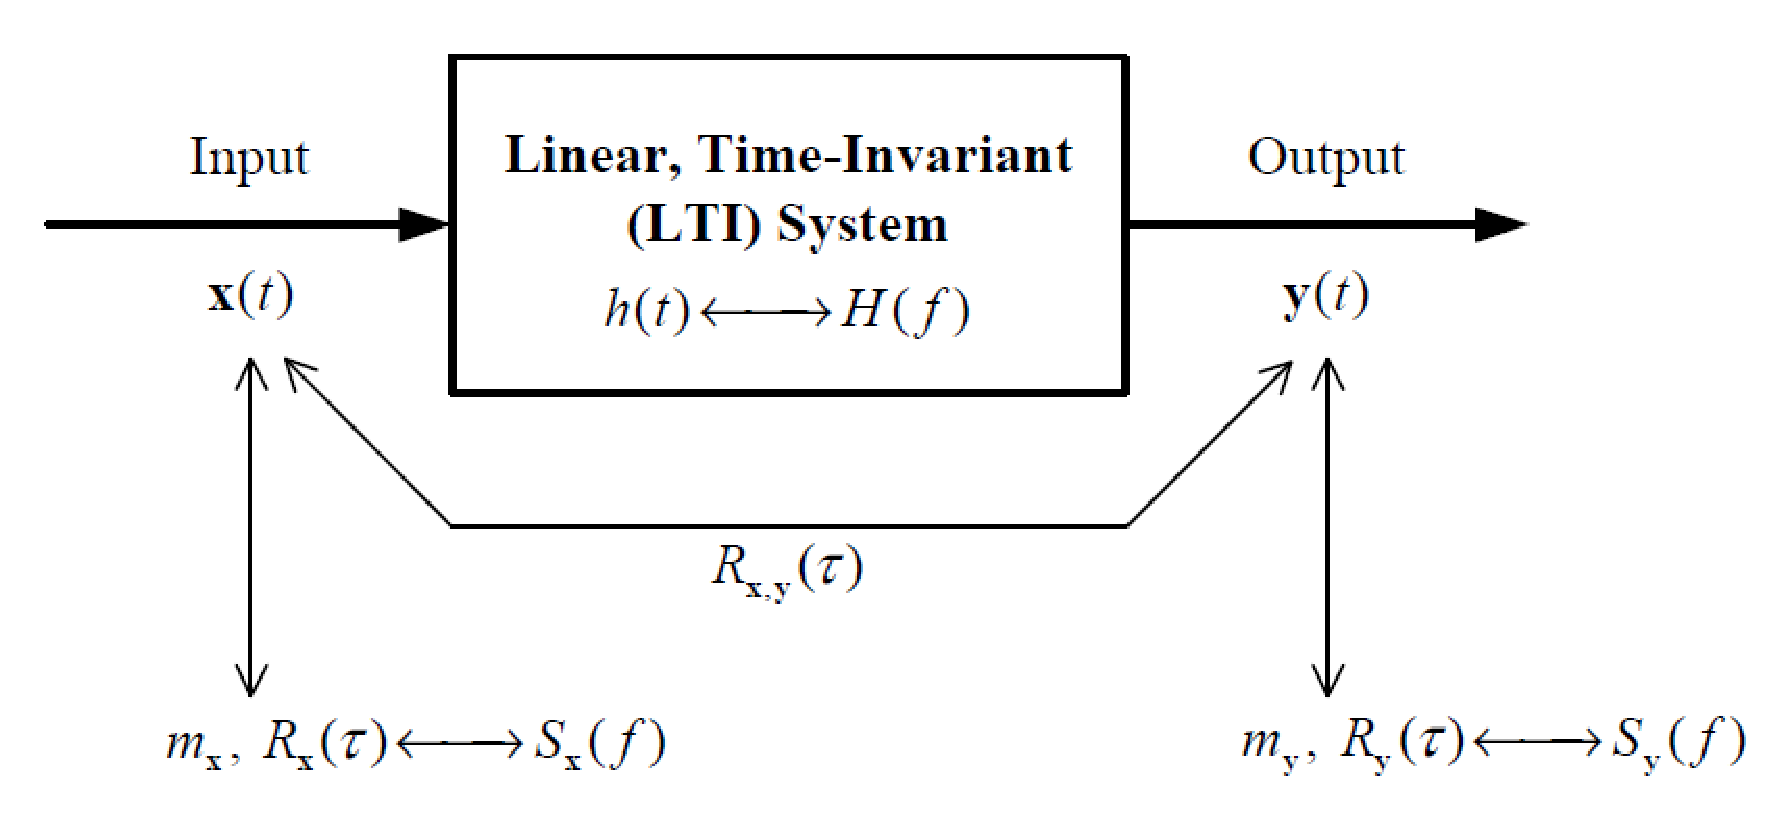
\includegraphics[width=0.7\columnwidth]{figs/fig26}
	  \end{center}
	\end{figure}
          
    \begin{align}
	  m_{\vay} &=  E\{\vay(t)\} = E\left\{ \int_{-\infty}^{\infty} h(\lambda)\vax(t-\lambda)\mathrm{d}\lambda \right\} = m_{\vax} H(0) \\
	  S_{\vay}(f) &= |H(f)|^2 S_{\vax}(f) \\
	  R_{\vay}(\tau) &= h(\tau) * h(-\tau) * R_{\vax}(\tau)
    \end{align}


\end{frame}
